\documentclass[math,code]{amznotes}
\setcounter{tocdepth}{2}  % Only show subsections and sections in the ToC
\usepackage{amsmath}
\usepackage{amsfonts}
\usepackage{graphicx}
\usepackage{tikz}
\usepackage{etoolbox}
\usepackage{tabularx}
\usepackage{float} % Needed for [H] placement specifier
\usepackage{wrapfig} % Needed for wrapping figures
\usepackage{diagbox} % For diagonal split in table
\usepackage{booktabs} % For better table formatting
\usepackage[normalem]{ulem} % For table usage
\useunder{\uline}{\ul}{} % For table usage
\usepackage{multirow} % For multirow
\usepackage{longtable} % For longtable

\graphicspath{ {./images/} }
\geometry{
    a4paper,
    headheight = 1.5cm
}

\patchcmd{\chapter}{\thispagestyle{plain}}{\thispagestyle{fancy}}{}{}

\theoremstyle{remark}
\newtheorem*{claim}{Claim}
\newtheorem*{remark}{Remark}
\newtheorem{case}{Case}

\newcommand{\entry}[5]{\markboth{#1}{#1}\textbf{#1}\ {(#2)}\ \textit{#3}\ $\bullet$\ \textbf{\textit{#4}} \begin{small}#5\end{small}}  % Defines the command to print each word on the page, \markboth{}{} prints the first word on the page in the top left header and the last word in the top right

%----------------------------------------------------------------------------------------

\begin{document}
\fancyhead[L]{
    French 5
}
\fancyhead[R]{
    Lecture Notes
}
\tableofcontents

\chapter{Unité 1}
\section{Le subjonctif présent}

En français, on utilise plusieurs structures impersonnelles\footnote{Par exemples, ``il est'' et ``c'est'' sont des structures impersonnelles, mais les structures avec \textit{``il est''} expriment une opinion \textbf{plus personnelle}, \textit{``c'est''} est utilisé pour \textbf{la généralité}.} avec \textit{il} suivies par le subjonctif.\footnote{Le \textit{il} ne représente personne et ne peut pas être changé par un autre pronom.} Par exemple, Il faut que, Il vaut mieux que\footnote{It is better that}, etc. Tout s'ajoute\footnote{adds itself with} \textbf{sujet + subjonctif}

\begin{notebox}
    \begin{remark}
    \textbf{Attention}:
    \begin{enumerate}
        \item Après une construction impersonnelle, il n'y a pas toujours le subjonctif. Il est aussi possible d'avoir l'indicatif.
        \begin{itemize}
            \item \textbf{Le subjonctif} est utilisé pour parler \textbf{d'une réalité incertaine}.
            \item \textbf{L'indicatif} pour \textbf{une réalité certaine} ou probable.
        \end{itemize}
        Et tous les cas sont les suivants,
        
        \centerline{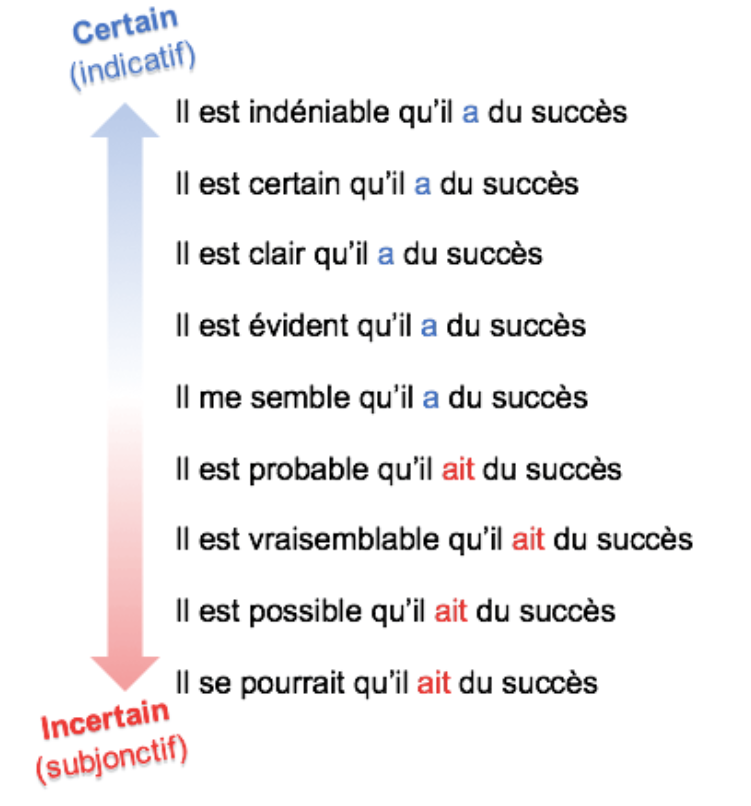
\includegraphics[width=0.5\linewidth]{images/1.png}}
    \end{enumerate}
    \end{remark}
\end{notebox}

\begin{enumerate}
    \item \textbf{Emploi}:
    \begin{itemize}
        \item Pour exprimer une action \textbf{éventuelle}\footnote{potential}, dont la réalisation n'est \textbf{pas certaine}.
        \item Une nécessité: Il est nécessaire que; il est indispensable que,; il faut que; il vaut mieux que; il est importante que;
        \item Une volonté\footnote{will}: vouloir, exiger\footnote{v. demand}, ordonner, désirer, demander, souhaiter, $\dots$ \\
        \centerline{Subject 1 + \textcolor{orange}{verb of volonté} + \textcolor{orange}{que} + Subject 2 + subjonctif} \\
        e.g., Je demande que tu viennes.
    \end{itemize}
    \item (\textbf{Conjugaison Règle}): 
    \begin{itemize}
        \item \textbf{Pour \textit{je, tu, il/elle/on, ils/elles} :} Prenez le radical de la $3^{\text{ème}}$ personne du pluriel (\textit{ils/elles}) du présent de l'indicatif (retirez \textit{-ent}) et ajoutez les terminaisons \textbf{-e, -es, -e, -ent}.
        \item \textbf{Pour \textit{nous, vous} :} Prenez le radical de la $1^{\text{ère}}$ personne du pluriel (\textit{nous}) du présent de l'indicatif (retirez \textit{-ons}) et ajoutez les terminaisons \textbf{-ions, -iez}.
    \end{itemize}
    \item (Des exemples)
    \begin{table}[h]
    \centering
    \begin{tabular}{|l|l|l|l|}
        \hline
        \textbf{Infinitif} & \textbf{Indicatif (3e pers. plur.)} & \textbf{Subjonctif (je)} & \textbf{Subjonctif (nous)} \\
        \hline
        Partir & Ils part\sout{ent} & que je part\textbf{e} & que nous part\textbf{ions} \\
        \hline
        Mettre & Ils mett\sout{ent} & que je mett\textbf{e} & que nous mett\textbf{ions} \\
        \hline
        Prendre & Ils prenn\sout{ent} & que je prenn\textbf{e} & que nous pren\textbf{ions} \\
        \hline
        Boire & Ils boiv\sout{ent} & que je boiv\textbf{e} & que nous buv\textbf{ions} \\
        \hline
        Venir & Ils vienn\sout{ent} & que je vienn\textbf{e} & que nous ven\textbf{ions} \\
        \hline
        Échanger & Ils échang\sout{ent} & que j'échang\textbf{e} & que nous échang\textbf{ions} \\
        \hline
        Connaître & Ils connaiss\sout{ent} & que je connaiss\textbf{e} & que nous connaiss\textbf{ions} \\
        \hline
        Attendre & Ils attend\sout{ent} & que j'attend\textbf{e} & que nous attend\textbf{ions} \\
        \hline
    \end{tabular}
    \end{table}
    \item (\textbf{Les irréguliers})
    \begin{center}
    \begin{longtable}{|c|c|c|c|c|}
    \caption{Verbes irréguliers au subjonctif} \\
    \hline
    \multicolumn{5}{|c|}{\textbf{\textcolor{blue}{Verbes irréguliers}}} \\
    \hline
    & \textbf{avoir} & \textbf{être} & \textbf{aller} & \textbf{faire} \\
    \hline
    \multirow{6}{*}{\textbf{que/qu'}} 
    & j'aie & je sois & j'aille & je fasse \\
    \cline{2-5}
    & tu aies & tu sois & tu ailles & tu fasses \\
    \cline{2-5}
    & il ait & il soit & il aille & il fasse \\
    \cline{2-5}
    & nous ayons & nous soyons & nous allions & nous fassions \\
    \cline{2-5}
    & vous ayez & vous soyez & vous alliez & vous fassiez \\
    \cline{2-5}
    & ils aient & ils soient & ils aillent & ils fassent \\
    \hline
    & \textbf{pouvoir} & \textbf{valoir} & \textbf{savoir} & \textbf{vouloir} \\
    \hline
    \multirow{6}{*}{\textbf{que/qu'}} 
    & je puisse & je vaille & je sache & je veuille \\
    \cline{2-5}
    & tu puisses & tu vailles & tu saches & tu veuilles \\
    \cline{2-5}
    & il puisse & il vaille & il sache & il veuille \\
    \cline{2-5}
    & nous puissions & nous valions & nous sachions & nous voulions \\
    \cline{2-5}
    & vous puissiez & vous valiez & vous sachiez & vous vouliez \\
    \cline{2-5}
    & ils puissent & ils vaillent & ils sachent & ils veuillent \\
    \hline
    \end{longtable}
    \end{center}
    \vspace{-30pt} % or -5pt or -8mm etc.
    \item Les exemples utiles:
    \begin{itemize}
        \item Il faut que nous \textbf{ne finissions pas} derniers.
        \item Il est indispensable que les candidats \textbf{convainquent} le jury.
    \end{itemize}
\end{enumerate}



\section{Les adjectifs et pronoms indéfinis}
Ils expriment une \textbf{certaine quantité}.

\begin{enumerate}
    \item \textbf{Les Adjectifs Indéfinis} (complètent un nom)
    \begin{itemize}
        \item \textbf{Aucun(e) \dots\ ne} ($0\%$) : \textit{Aucun apprenant\footnote{n. learner} n'a fait son travail.}
        \item \textbf{Quelques} ($\approx 25\%$) : \textit{Quelques apprenants l'ont fait.}
        \item \textbf{Plusieurs} ($\approx 75\%$) : \textit{Plusieurs apprenants l'ont fait.}
        \item \textbf{Tout / Tous / Toute / Toutes} ($100\%$) : \textit{Tous les apprenants ont fait leur travail.}
    \end{itemize}

    \item \textbf{Les Pronoms Indéfinis} (remplacent un nom)
    \begin{itemize}
        \item \textbf{Tous / Toutes} : \textit{Ils ont \textbf{tous} fait leur travail.} (remplace la totalité du groupe)
        \item \textbf{Aucun(e)}: J'ai invité plusieurs personnes, mais \textbf{aucune} n'est venue.
        \item \textbf{Certains / Certaines} : \textit{\textbf{Certains} l'ont fait\dots} (remplace une partie du groupe)
        \item \textbf{D'autres} : \textit{\dots\ et \textbf{d'autres}, non.} (remplace le reste du groupe)
        \item \textbf{Beaucoup}: il signifie \textbf{un grand nombre}.
        \item \textbf{Chacun / Chacune}\footnote{each} : \textit{\textbf{Chacun(e)} a eu un travail à faire.} (remplace chaque élément individuellement)
        \item \textbf{Quelqu'un / Quelques-uns / Quelques-unes} : \textit{Il n'en reste plus que \textbf{quelques-uns}.} (remplace une petite quantité indéterminée)
    \end{itemize}

    \begin{notebox}
        Remark. Le regle utile est:
        \begin{enumerate}
            \item First, decide: noun or no noun?
            \item Then find the meaning using the following information:
            \begin{itemize}
                \item \textbf{0} $\rightarrow$ \textit{aucun(e)}
                \item \textbf{a few / some} $\rightarrow$ \textit{quelques / quelques-uns}
                \item \textbf{several} $\rightarrow$ \textit{plusieurs}
                \item \textbf{some of the group} $\rightarrow$ \textit{certains}
                \item \textbf{the others} $\rightarrow$ \textit{d'autres}
                \item \textbf{many / a lot} $\rightarrow$ \textit{beaucoup}
                \item \textbf{all} $\rightarrow$ \textit{tous / toutes}
                \item \textbf{each one} $\rightarrow$ \textit{chacun / chacune}
                \item \textbf{someone} $\rightarrow$ \textit{quelqu'un}
            \end{itemize}
        \end{enumerate}
    \end{notebox}
\end{enumerate}

\chapter{Unité 2}

\section{L'accord du participe passe}
\label{sec:l'accord-du-pp}

\begin{enumerate}
    \item Avec \textcolor{orange}{\^etre} : le participe passé s'accorde avec le sujet.
    \begin{itemize}
        \item La directrice \textcolor{orange}{s'est énervée} car deux de ses employés \textcolor{orange}{se sont endormis} pendant une réunion de travail.
        \item 2210 établissements\footnote{institutions} \textcolor{orange}{se sont inscrits}.
        \item Elles \textcolor{orange}{sont sorties} de la maison.
        \item Vous \textcolor{orange}{êtes rentré(e)(s)} tard hier soir.
        \item Pendant qu'elle \textcolor{orange}{dormait}, quelqu'un \textcolor{orange}{est entré}.
        \item Je \textcolor{orange}{regardais} la télévision quand tu \textcolor{orange}{m'as appelé(e)}.
    \end{itemize}

    \begin{notebox}
        \textbf{Quels verbes utilisent être ? --- DR \& MRS VANDERTRAMP}
        
        Au passé composé, certains verbes de mouvement ou de changement d'état
        utilisent \textbf{être}. On peut retenir :
        
        \begin{itemize}
            \item \textbf{D} --- devenir
            \item \textbf{R} --- revenir
            \item \textbf{M} --- monter
            \item \textbf{R} --- rentrer
            \item \textbf{S} --- sortir
            \item \textbf{V} --- venir
            \item \textbf{A} --- aller
            \item \textbf{N} --- naître
            \item \textbf{D} --- descendre
            \item \textbf{E} --- entrer
            \item \textbf{R} --- retourner
            \item \textbf{T} --- tomber
            \item \textbf{R} --- rester
            \item \textbf{A} --- arriver
            \item \textbf{M} --- mourir
            \item \textbf{P} --- partir
        \end{itemize}
        
        Les \textbf{verbes pronominaux} utilisent aussi toujours \textbf{être} :
        \textit{se lever, se tourner, s'endormir, s'inscrire, \dots}
        
        \textbf{Attention :} certains de ces verbes peuvent utiliser \textbf{avoir}
        quand ils ont un COD : \textit{Elle est sortie.} mais
        \textit{Elle a sorti la voiture.}
    \end{notebox}


    \item Avec \textcolor{orange}{avoir} : le participe passé s'accorde avec le COD s'il est placé avant.
    \begin{itemize}
        \item L'entreprise a créé une salle de repos qu'ils \textcolor{orange}{ont installée} au dernier étage.
    \end{itemize} 

    \item \textbf{Méthode pour faire l'accord du participe passé}
    \begin{enumerate}
        \item Trouver d'abord \textbf{l'auxiliaire} : \textit{être} ou \textit{avoir}.
        
        \item Si c'est \textbf{être} :
        \begin{itemize}
            \item Le participe passé s'accorde généralement avec le \textbf{sujet}.
            \item \textit{Céline s'est \textcolor{orange}{tournée}.}
            \quad Céline = féminin singulier $\rightarrow$ \textit{-ée}.
        \end{itemize}
        
        \item Si c'est \textbf{avoir} :
        \begin{itemize}
            \item Chercher le \textbf{COD} : poser la question
            \textit{qui ? / quoi ?} après le verbe.
            \item COD \textbf{après} le verbe $\rightarrow$ \textbf{pas d'accord}.
            \item COD \textbf{avant} le verbe $\rightarrow$ accord avec le COD.
        \end{itemize}
        
        \begin{itemize}
            \item \textit{Mme Lambert a \textcolor{orange}{licencié} un employé.}
            \quad COD après $\rightarrow$ pas d'accord.
            
            \item \textit{La DRH a appelé Marion et elle l'a
            \textcolor{orange}{convoquée}.}
            \quad \textit{l'} = Marion, COD avant $\rightarrow$ féminin singulier.
            
            \item \textit{Les lettres qu'il a
            \textcolor{orange}{envoyées}.}
            \quad \textit{que} = les lettres, COD avant $\rightarrow$ féminin pluriel.
        \end{itemize}
        
        \item Si le pronom est un \textbf{COI}\footnote{Complément d'objet indirect, usually with a preposition such as à} (\textit{lui, leur, \dots}),
        il ne provoque pas l'accord.
        \begin{itemize}
            \item \textit{Je \textbf{leur} ai \textcolor{orange}{annoncé} que\dots}
            \quad \textit{leur} = COI $\rightarrow$ pas d'accord.
        \end{itemize}
    \end{enumerate}

    \begin{notebox}
        \textbf{Comment former le participe passé ?}
        
        Pour former le participe passé d'un verbe :
        
        \begin{itemize}
            \item \textbf{-er} $\rightarrow$ \textbf{-é} : \textit{aimer $\rightarrow$ aimé}
            \item \textbf{-ir} $\rightarrow$ \textbf{-i} : \textit{finir $\rightarrow$ fini}
            \item \textbf{-re} $\rightarrow$ souvent \textbf{-u} : \textit{vendre $\rightarrow$ vendu}
        \end{itemize}
        
        \textbf{Attention :} il existe des participes passés irréguliers qu'il faut apprendre :
        \textit{faire $\rightarrow$ fait, prendre $\rightarrow$ pris, recevoir $\rightarrow$ reçu,
        écrire $\rightarrow$ écrit, voir $\rightarrow$ vu, mettre $\rightarrow$ mis, 
        venir $\rightarrow$ venu, ouvrir $\rightarrow$ ouvert, être $\rightarrow$ été, vivre $\rightarrow$ vecu
        devoir $\rightarrow$ dû, savoir $\rightarrow$ su, lire $\rightarrow$ lu}
    \end{notebox}

    \item À la voix passive : \textcolor{orange}{être + participe passé}. Le participe passé s'accorde avec le sujet.
    \begin{itemize}
        \item La maison vient tout juste d'\textcolor{orange}{être restaurée}.
        \item Le papier peint a été \textcolor{orange}{recréé} à l'identique.
        \item Les meubles d'origine ont été \textcolor{orange}{recherchés} et \textcolor{orange}{rachetés}.
        \item Certains ont été \textcolor{orange}{trouvés} dans le village même.
        \item Le piano est celui qui a été \textcolor{orange}{décrit} par Colette.
        \item Les meubles étaient un peu \textcolor{orange}{éparpillés} dans toute la France.
        \item Tout a été \textcolor{orange}{reconstruit} à l'identique.
    \end{itemize}

    \item \textbf{Imparfait ou passé composé ?}
    
    \begin{itemize}
        \item On utilise \textcolor{orange}{l'imparfait} pour une action ou une situation
        qui a une certaine \textbf{durée} dans le passé :
        \begin{itemize}
            \item \textbf{Description / situation} :
            \textit{Il faisait beau et la ville était calme.}
            \item \textbf{Habitude / répétition} :
            \textit{Quand j'étais petit, je jouais au football tous les jours.}
            \item \textbf{Action en cours / simultanéité} :
            \textit{Je regardais la télévision pendant qu'elle travaillait.}
        \end{itemize}
    
        \item On utilise le \textcolor{orange}{passé composé} pour une action
        \textbf{ponctuelle, terminée ou soudaine} :
        \begin{itemize}
            \item \textbf{Action ponctuelle / terminée} :
            \textit{Hier, j'ai acheté un livre.}
            \item \textbf{Action soudaine} :
            \textit{Je dormais quand le téléphone a sonné.}
            \item \textbf{Suite d'actions / énumération} :
            \textit{Je suis arrivé, j'ai mangé et je suis parti.}
        \end{itemize}
    \end{itemize}
    
    \begin{notebox}
    \textbf{Comment conjuguer l'imparfait ?}
    
    On prend la forme de \textbf{nous au présent}, on enlève \textbf{-ons},
    puis on ajoute :
    
    \[
    \boxed{-ais,\ -ais,\ -ait,\ -ions,\ -iez,\ -aient}
    \]
    
    Par exemple, avec \textit{boire} :
    
    \[
    \text{nous buvons} \rightarrow \text{buv-}
    \]
    
    \begin{itemize}
        \item je buvais
        \item tu buvais
        \item il / elle buvait
        \item nous buvions
        \item vous buviez
        \item ils / elles buvaient
    \end{itemize}
    
    \textbf{Exception principale : être}
    \[
    \text{être} \rightarrow \text{ét-}
    \]
    \textit{j'étais, tu étais, il était, nous étions, vous étiez, ils étaient.}
    
    \textbf{Attention à l'orthographe :}
    \begin{itemize}
        \item verbes en \textbf{-ger} : \textit{manger $\rightarrow$ je mangeais},
        mais \textit{nous mangions}.
        \item verbes en \textbf{-cer} : \textit{commencer $\rightarrow$ je commençais},
        mais \textit{nous commencions}.
    \end{itemize}
    \end{notebox}
    
    \begin{notebox}
    \textbf{Astuce :} dans une histoire, l'\textbf{imparfait} donne souvent
    le \textbf{contexte / l'action en cours}, tandis que le \textbf{passé composé}
    indique l'\textbf{événement qui arrive}.
    
    \[
    \underbrace{\text{Je dormais}}_{\text{action en cours}}
    \quad\text{quand}\quad
    \underbrace{\text{le téléphone a sonné.}}_{\text{événement ponctuel}}
    \]
    \end{notebox}
\end{enumerate}

\section{La place et la forme des adjectifs}

\begin{enumerate}
    \item \textcolor{orange}{Après le nom} : en général, la majorité des adjectifs se placent après le nom.
    \begin{itemize}
        \item Les adjectifs de \textbf{couleur} : des uniformes \textcolor{orange}{bleu marine}.
        \item Les adjectifs de \textbf{nationalité} : des collègues \textcolor{orange}{espagnols}.
        \item Les adjectifs de \textbf{forme} et beaucoup d'autres adjectifs : une tête \textcolor{orange}{coiffée}\footnote{a styled head}.
    \end{itemize}
    
    \item \textcolor{orange}{Avant le nom} : certains adjectifs très courants se placent généralement avant le nom.
    \begin{itemize}
        \item On peut retenir la règle \textbf{BRAGS} :
        \begin{itemize}
            \item \textbf{B -- Beauty} : beau, joli $\dots$
            \item \textbf{R -- Rank} : premier, dernier, prochain $\dots$
            \item \textbf{A -- Age} : jeune, vieux, nouveau, ancien $\dots$
            \item \textbf{G -- Goodness} : bon, mauvais $\dots$
            \item \textbf{S -- Size} : petit, grand, gros $\dots$
        \end{itemize}
        \item Les nombres se placent aussi devant le nom : \textit{deux dossiers, trois étudiants, le deuxième exercice}.
    \end{itemize}

    \begin{notebox}
        \begin{enumerate}
            \item \textbf{S'il y a plusieurs adjectifs,} chaque adjectif garde généralement sa place normale :
            \begin{itemize}
                \item de \textcolor{orange}{jeunes} collègues \textcolor{orange}{espagnols}
                \item ces \textcolor{orange}{deux autres} dossiers \textcolor{orange}{rouges}
                \item un collaborateur \textcolor{orange}{sympa} avec de \textcolor{orange}{vraies}\footnote{true, genuine} compétences
            \end{itemize}
            Donc, les adjectifs ne doivent pas nécessairement être tous avant ou tous après le nom.
            \item \textbf{Devant une voyelle ou un ``h'' muet,} ``beau'', ``vieux'', ``nouveau'' deviennent ``bel'', ``vieil'', ``nouvel''!
        \end{enumerate}
        
    \end{notebox}

    \item \textcolor{orange}{Avant ou après} : le sens change.
    \begin{itemize}
        \item \textbf{ancien}: avant = former; après = old/ancient
        \item \textbf{cher}: avant = dear/beloved; après = expensive
        \item \textbf{curieux}: avant = strange/unusual; après = curious/inquisitive
        \item \textbf{drôle}: avant = strange/odd; après = funny/amusing
        \item \textbf{pauvre}: avant = unfortunate/pitiful; après = poor/not wealthy
        \item \textbf{grand}: avant = great/important; après = big/tall
        \item \textbf{sale}: avant = nasty/unpleasant; après = dirty
        \item \textbf{simple}: avant = mere/just; après = simple/uncomplicated
        \item \textbf{vrai}: avant = real/genuine; après = true/factually correct
    \end{itemize}

    \begin{notebox}
        Qu'il soit placé avant ou après le nom, l'adjectif s'accorde \textbf{toujours} en genre et en nombre avec le nom (ou le sujet).
    \end{notebox}

    \item Un adjectif peut être \textcolor{orange}{un participe passé}.
    \begin{itemize}
        \item Une fois la lecture du dossier \textcolor{orange}{terminée}, vous pourrez venir me voir.
        \item Les fenêtres \textcolor{orange}{ouvertes} laissaient passer un léger vent.
    \end{itemize}
\end{enumerate}

\chapter{Unité 3}

\section{Le gérondif}

Le gérondif est une forme verbale qui permet de relier deux actions. Il se forme avec \textbf{en + participe présent} (verbe en \textit{-ant}).

\subsection*{Quand utiliser le gérondif ?}

Le gérondif peut exprimer plusieurs idées :

\begin{enumerate}
    \item \textbf{La simultanéité} : deux actions se passent en même temps.\footnote{Two actions happen at the same time.}
    \begin{itemize}
        \item Je mange en regardant la télévision.
        \item Elle écoute de la musique en faisant ses devoirs.
    \end{itemize}

    \item \textbf{La manière} : il explique comment on fait quelque chose.\footnote{It explains how an action is performed.}
    \begin{itemize}
        \item J'apprends le français en parlant avec mes amis.
        \item Il reste en forme en faisant du sport.
    \end{itemize}

    \item \textbf{La cause} : il explique pourquoi quelque chose se passe.\footnote{It expresses the reason or cause of an action.}
    \begin{itemize}
        \item En travaillant trop, il est devenu fatigué.
        \item En mangeant trop vite, j'ai eu mal au ventre.
    \end{itemize}

    \item \textbf{La condition} : il exprime une condition, comme avec \textit{si}.\footnote{It expresses a condition, similar to ``if'' in English.}
    \begin{itemize}
        \item En étudiant régulièrement, tu réussiras ton examen.
        \item En partant maintenant, nous arriverons à l'heure.
    \end{itemize}
\end{enumerate}

\begin{notebox}
    On peut ajouter \textbf{tout} devant le gérondif pour insister sur la simultanéité ou pour exprimer une opposition.\footnote{Adding ``tout'' emphasizes simultaneity or can express contrast, similar to ``even though''.}
    \begin{itemize}
        \item Elle parle tout en mangeant. (simultanéité)
        \item Il a réussi son examen tout en travaillant à temps partiel. (opposition)
    \end{itemize}
\end{notebox}

\subsection*{Comment former le gérondif ?}

Pour former le gérondif, on utilise le radical de la première personne du pluriel (\textit{nous}) au présent, on enlève \textit{-ons} et on ajoute \textbf{en + -ant}.

\begin{center}
    \textbf{nous + verbe au présent}
    $\longrightarrow$ \textbf{radical + -ant}
    $\longrightarrow$ \textbf{en + participe présent}
\end{center}

\begin{itemize}
    \item Parler : nous parlons $\rightarrow$ en parlant
    \item Finir : nous finissons $\rightarrow$ en finissant
    \item Prendre : nous prenons $\rightarrow$ en prenant
    \item Faire : nous faisons $\rightarrow$ en faisant
    \item Écrire : nous écrivons $\rightarrow$ en écrivant
    \item Venir : nous venons $\rightarrow$ en venant
    \item Se mettre : nous nous mettons $\rightarrow$ en se mettant
\end{itemize}

\begin{notebox}
    \textbf{Attention :} Le sujet du gérondif est normalement le même que celui du verbe principal.\footnote{The gerund and the main verb normally have the same subject.}
    \begin{itemize}
        \item Je révise mes cours en écoutant de la musique.
        \item Elle a rencontré ses amis en allant à l'université.
    \end{itemize}
\end{notebox}

\subsection*{Les verbes irréguliers}

Il existe seulement \textbf{trois verbes irréguliers} au participe présent :

\begin{center}
\begin{tabular}{ll}
    \hline
    \textbf{Verbe} & \textbf{Gérondif} \\
    \hline
    Être & en étant \\
    Avoir & en ayant \\
    Savoir & en sachant \\
    \hline
\end{tabular}
\end{center}

\textbf{Exemples :}
\begin{itemize}
    \item En étant bien organisé, je gagne du temps.
    \item En ayant plus de temps libre, je pourrais faire du sport.
    \item En sachant parler français, tu peux communiquer avec plus de personnes.
\end{itemize}


\section{La cause et la conséquence}

Une \textbf{cause} explique pourquoi une action se passe, tandis qu'une \textbf{conséquence} explique le résultat de cette action.\footnote{A cause explains why something happens, while a consequence describes its result.}

\subsection*{Exprimer la cause}

Pour exprimer la cause, on utilise plusieurs expressions :

\begin{enumerate}
    \item \textbf{Parce que / Car} : pour donner une raison.\footnote{Because / since. ``Car'' is generally more formal and is used to connect two clauses.}
    \begin{itemize}
        \item Je reste à la maison parce que je suis malade.
        \item Je ne peux pas sortir, car j'ai beaucoup de travail.
    \end{itemize}

    \item \textbf{Comme} : pour présenter la cause au début de la phrase.\footnote{Since / as. ``Comme'' is usually placed at the beginning of the sentence.}
    \begin{itemize}
        \item Comme il pleut, je prends mon parapluie.
        \item Comme je suis fatigué, je vais me coucher tôt.
    \end{itemize}

    \item \textbf{Puisque / Étant donné que} : pour présenter une raison déjà connue ou évidente.\footnote{Since / given that. These expressions often introduce a reason that is already known or accepted.}
    \begin{itemize}
        \item Puisque tu es libre, nous pouvons aller au cinéma.
        \item Étant donné qu'il pleut, nous restons à la maison.
    \end{itemize}

    \item \textbf{Grâce à + nom} : pour exprimer une cause positive.\footnote{Thanks to. Generally used for a positive cause.}
    \begin{itemize}
        \item Grâce à mes amis, j'ai réussi mon examen.
        \item Grâce à Internet, nous pouvons apprendre facilement.
    \end{itemize}

    \item \textbf{À cause de + nom} : pour exprimer une cause négative.\footnote{Because of / due to. Generally used for a negative cause.}
    \begin{itemize}
        \item À cause de la pluie, je suis arrivé en retard.
        \item À cause du bruit, je ne peux pas dormir.
    \end{itemize}
\end{enumerate}

\begin{notebox}
\textbf{Attention :} On utilise \textbf{parce que, car, comme, puisque, étant donné que + proposition} (sujet + verbe), mais \textbf{grâce à / à cause de + nom}.

\begin{itemize}
    \item Je suis en retard parce qu'il pleut.
    \item Je suis en retard à cause de la pluie.
\end{itemize}

\textbf{Remarque :} Devant une voyelle, \textit{parce que} devient \textit{parce qu'}, et \textit{à cause de} devient \textit{à cause d'}.
\end{notebox}

\subsection*{Exprimer la conséquence}

Pour exprimer la conséquence, on utilise plusieurs expressions :

\begin{enumerate}
    \item \textbf{Donc / Alors} : pour présenter un résultat.\footnote{Therefore / so. Common in both spoken and written French.}
    \begin{itemize}
        \item Je suis malade, donc je reste à la maison.
        \item Il pleut, alors nous ne sortons pas.
    \end{itemize}

    \item \textbf{Du coup} : pour exprimer une conséquence à l'oral.\footnote{So / as a result. Very common in informal spoken French.}
    \begin{itemize}
        \item J'ai raté mon bus. Du coup, je suis arrivé en retard.
    \end{itemize}

    \item \textbf{C'est pourquoi / Par conséquent} : pour exprimer une conséquence, surtout à l'écrit.\footnote{That is why / consequently. More formal than ``du coup''.}
    \begin{itemize}
        \item Je veux améliorer mon français. C'est pourquoi je pratique tous les jours.
        \item Il n'a pas étudié. Par conséquent, il a échoué à son examen.
    \end{itemize}

    \item \textbf{Si bien que} : pour introduire directement une conséquence.\footnote{So that / with the result that.}
    \begin{itemize}
        \item Il a beaucoup travaillé, si bien qu'il est très fatigué.
    \end{itemize}

    \item \textbf{Tellement + adjectif / adverbe + que} : pour exprimer une conséquence liée à une forte intensité.\footnote{So + adjective/adverb + that.}
    \begin{itemize}
        \item Je suis tellement fatigué que je ne peux pas travailler.
        \item Il parle tellement vite que je ne comprends rien.
    \end{itemize}

    \item \textbf{Tellement de + nom + que} : pour exprimer une conséquence liée à une grande quantité.\footnote{So much / so many + noun + that.}
    \begin{itemize}
        \item J'ai tellement de devoirs que je ne peux pas sortir.
    \end{itemize}
\end{enumerate}

On peut aussi utiliser des \textbf{verbes} pour exprimer la conséquence : \textit{provoquer, entraîner, causer, déclencher}.\footnote{To provoke, lead to, cause, trigger.}

\begin{itemize}
    \item Le stress peut provoquer des problèmes de santé.
    \item La pollution entraîne des problèmes environnementaux.
    \item La pluie a causé un accident.
\end{itemize}

\begin{notebox}
\textbf{Remarque :} Certaines expressions sont plus utilisées à l'oral ou à l'écrit.

\begin{itemize}
    \item \textbf{À l'oral :} alors, donc, du coup.
    \item \textbf{À l'écrit :} donc, c'est pourquoi, par conséquent, si bien que.
\end{itemize}

\textbf{Attention :} Avec \textit{tellement ... que}, on utilise l'indicatif pour exprimer une conséquence réelle.

\begin{itemize}
    \item Il est tellement occupé qu'il n'a pas le temps de manger.
\end{itemize}
\end{notebox}

\subsection*{La différence entre la cause et la conséquence}

On peut exprimer la même idée avec la cause ou la conséquence.

\begin{itemize}
    \item \textbf{Cause :} Je reste à la maison parce que je suis malade.
    \item \textbf{Conséquence :} Je suis malade, donc je reste à la maison.
\end{itemize}

\begin{itemize}
    \item \textbf{Cause :} Comme il pleut, nous ne sortons pas.
    \item \textbf{Conséquence :} Il pleut, c'est pourquoi nous ne sortons pas.
\end{itemize}

\chapter{Unité 4}

\section{Les pronoms relatifs}

Les \textbf{pronoms relatifs} permettent de relier deux phrases et de remplacer un nom pour éviter une répétition.\footnote{Relative pronouns connect two clauses and replace a noun to avoid repetition.}

Il existe quatre pronoms relatifs principaux : \textbf{qui, que, où et dont}.

\subsection*{Quand utiliser les pronoms relatifs ?}

\begin{enumerate}
    \item \textbf{Qui} : remplace le sujet d'un verbe.\footnote{Who / which / that. Used when the relative pronoun is the subject of the following verb.}
    \begin{itemize}
        \item J'ai un ami. Il parle français.
        \item $\rightarrow$ J'ai un ami \textbf{qui} parle français.
        \item C'est un livre \textbf{qui} est très intéressant.
    \end{itemize}

    \item \textbf{Que / Qu'} : remplace le complément d'objet direct (COD) d'un verbe.\footnote{Whom / which / that. Used when the relative pronoun is the direct object of the following verb.}
    \begin{itemize}
        \item J'ai acheté un livre. Tu aimes ce livre.
        \item $\rightarrow$ J'ai acheté un livre \textbf{que} tu aimes.
        \item C'est le film \textbf{qu'}il regarde.
    \end{itemize}

    \item \textbf{Où} : remplace un complément de lieu ou de temps.\footnote{Where / when. Used to refer to a place or a time.}
    \begin{itemize}
        \item C'est la ville. Je suis né dans cette ville.
        \item $\rightarrow$ C'est la ville \textbf{où} je suis né.
        \item C'est le jour \textbf{où} nous nous sommes rencontrés.
    \end{itemize}

    \item \textbf{Dont} : remplace un complément introduit par \textit{de}.\footnote{Of which / whose / about which. Used to replace a complement introduced by ``de''.}
    \begin{itemize}
        \item Je connais une association. Tu parles de cette association.
        \item $\rightarrow$ Je connais une association \textbf{dont} tu parles.
        \item C'est le livre \textbf{dont} j'ai besoin.
    \end{itemize}
\end{enumerate}

\begin{notebox}
\textbf{Attention : Accord du participe passé avec \textit{que}}

Quand on utilise \textbf{que} comme pronom relatif avec un verbe au \textbf{passé composé} construit avec \textit{avoir}, le participe passé s'accorde en genre et en nombre avec le COD placé avant le verbe.\footnote{When the direct object comes before a verb using avoir in the passé composé, the past participle agrees with that object in gender and number.}

\begin{itemize}
    \item \textbf{Masculin singulier :} Le livre que j'ai lu.
    \item \textbf{Féminin singulier :} La photo que j'ai prise.
    \item \textbf{Masculin pluriel :} Les livres que j'ai lus.
    \item \textbf{Féminin pluriel :} Les photos que j'ai prises.
\end{itemize}

\textbf{Comparaison :}
\begin{itemize}
    \item J'ai \textbf{pris} une photo. (COD après le verbe : pas d'accord)
    \item La photo que j'ai \textbf{prise}. (COD avant le verbe : accord avec \textit{photo})
\end{itemize}

\textbf{Remarque :} Cet accord concerne le COD, pas le sujet. Avec \textit{qui}, il n'y a pas d'accord avec le nom précédent pour cette raison. Revisitez les notes \ref{sec:l'accord-du-pp}.
\end{notebox}


\subsection*{Comment utiliser \textit{dont} ?}

Le pronom relatif \textbf{dont} est utilisé quand un verbe, un adjectif ou un nom est construit avec la préposition \textbf{de}.

\begin{enumerate}
    \item \textbf{Avec un verbe + de}
    \begin{itemize}
        \item \textbf{Parler de} : C'est un sujet \textbf{dont} nous parlons.
        \item \textbf{Avoir besoin de} : Voici les documents \textbf{dont} j'ai besoin.
        \item \textbf{Rêver de} : C'est le voyage \textbf{dont} je rêve.
        \item \textbf{Se souvenir de} : C'est une histoire \textbf{dont} je me souviens.
    \end{itemize}

    \item \textbf{Avec un adjectif + de}
    \begin{itemize}
        \item \textbf{Être fier de} : C'est un projet \textbf{dont} je suis fier.
        \item \textbf{Être content de} : C'est un résultat \textbf{dont} je suis content.
    \end{itemize}

    \item \textbf{Avec un nom + de} : pour exprimer une relation ou une possession.\footnote{Used to express a relationship or possession, similar to ``whose''.}
    \begin{itemize}
        \item Je connais un homme. Son fils est médecin.
        \item $\rightarrow$ Je connais un homme \textbf{dont} le fils est médecin.
        \item C'est un livre \textbf{dont} la couverture est rouge.
    \end{itemize}

    \item \textbf{Pour exprimer une partie d'un ensemble} : \textit{dont} peut signifier \textit{parmi lesquels}.\footnote{Including / among which. Used to introduce part of a group.}
    \begin{itemize}
        \item Il y a plusieurs déchets, \textbf{dont} les nanoplastiques.
        \item J'ai visité trois pays, \textbf{dont} la France.
    \end{itemize}
\end{enumerate}

\begin{notebox}
\textbf{Attention :} Quand on utilise \textbf{dont}, on ne répète pas la préposition \textbf{de} dans la proposition relative.

\begin{itemize}
    \item Correct : C'est le livre \textbf{dont} j'ai besoin.
    \item Incorrect : C'est le livre \textbf{dont} j'ai besoin de.
\end{itemize}

\textbf{Remarque :} Avec \textit{dont}, la préposition \textit{de} fait déjà partie du pronom relatif.
\end{notebox}

\subsection*{Comment choisir le bon pronom relatif ?}

Pour choisir le bon pronom, on peut suivre ces étapes :

\begin{enumerate}
    \item \textbf{Le nom remplacé est-il le sujet du verbe ?}
    \begin{itemize}
        \item Oui $\rightarrow$ \textbf{qui}
        \item Exemple : La fille \textbf{qui} parle est mon amie.
    \end{itemize}

    \item \textbf{Le nom remplacé est-il le COD du verbe ?}
    \begin{itemize}
        \item Oui $\rightarrow$ \textbf{que}
        \item Exemple : La fille \textbf{que} je connais est gentille.
    \end{itemize}

    \item \textbf{Le nom remplacé indique-t-il un lieu ou un moment ?}
    \begin{itemize}
        \item Oui $\rightarrow$ \textbf{où}
        \item Exemple : C'est le restaurant \textbf{où} nous mangeons.
    \end{itemize}

    \item \textbf{Le nom remplacé est-il lié à une construction avec \textit{de} ?}
    \begin{itemize}
        \item Oui $\rightarrow$ \textbf{dont}
        \item Exemple : C'est le projet \textbf{dont} je suis fier.
    \end{itemize}
\end{enumerate}

\begin{notebox}
\textbf{Résumé :}

\begin{itemize}
    \item \textbf{Qui} $\rightarrow$ sujet.
    \item \textbf{Que} $\rightarrow$ complément d'objet direct (COD).
    \item \textbf{Où} $\rightarrow$ lieu ou temps.
    \item \textbf{Dont} $\rightarrow$ complément introduit par \textit{de}, ou partie d'un ensemble.
\end{itemize}

\textbf{Astuce :} Pour trouver le bon pronom relatif, reconstruisez les deux phrases originales et regardez la fonction du nom répété.\footnote{Reconstruct the two original sentences and identify the grammatical role of the repeated noun.}
\end{notebox}


\section{Le plus-que-parfait}

Le \textbf{plus-que-parfait} est un temps du passé qui permet d'exprimer une action qui s'est passée \textbf{avant une autre action passée}.\footnote{The plus-que-parfait (pluperfect) describes an action that happened before another past action. It is similar to ``had + past participle'' in English.}

\subsection*{Quand utiliser le plus-que-parfait ?}

Le plus-que-parfait exprime une \textbf{antériorité dans le passé}.\footnote{An action that happened earlier than another past action.}

\begin{enumerate}
    \item \textbf{Exprimer une action antérieure à une autre action passée}
    \begin{itemize}
        \item Quand je suis arrivé, le film \textbf{avait déjà commencé}.
        \item Elle \textbf{avait fini} ses devoirs avant de sortir.
        \item J'ai retrouvé le livre que j'\textbf{avais perdu}.
    \end{itemize}

    \item \textbf{Expliquer la cause d'une situation passée}
    \begin{itemize}
        \item J'étais fatigué parce que j'\textbf{avais mal dormi}.
        \item Il était triste parce qu'il \textbf{avait perdu} son téléphone.
    \end{itemize}

    \item \textbf{Raconter un événement passé dans un récit}\footnote{To describe an earlier event when telling a story about the past.}
    \begin{itemize}
        \item Hier, j'ai rencontré un ami que je n'\textbf{avais pas vu} depuis longtemps.
        \item Elle a réussi son examen parce qu'elle \textbf{avait beaucoup étudié}.
    \end{itemize}
\end{enumerate}

\begin{notebox}
\textbf{Attention :} Le plus-que-parfait s'utilise généralement avec un autre temps du passé, comme le \textbf{passé composé} ou l'\textbf{imparfait}.

\begin{itemize}
    \item \textbf{Plus-que-parfait} : action la plus ancienne.
    \item \textbf{Passé composé} : action passée terminée.
    \item \textbf{Imparfait} : description, habitude ou situation dans le passé.
\end{itemize}

\textbf{Exemple :} Quand je suis arrivé (passé composé), mes amis \textbf{avaient déjà mangé} (plus-que-parfait).

Cela signifie que mes amis ont mangé \textbf{avant} mon arrivée.
\end{notebox}

\subsection*{Comment former le plus-que-parfait ?}

Le plus-que-parfait se forme avec \textbf{avoir} ou \textbf{être} à l'imparfait + \textbf{participe passé}.

\begin{center}
    \textbf{Sujet + avoir / être (imparfait) + participe passé}
\end{center}

\begin{enumerate}
    \item \textbf{Avec l'auxiliaire avoir}
    \begin{itemize}
        \item J'\textbf{avais} mangé
        \item Tu \textbf{avais} mangé
        \item Il / Elle \textbf{avait} mangé
        \item Nous \textbf{avions} mangé
        \item Vous \textbf{aviez} mangé
        \item Ils / Elles \textbf{avaient} mangé
    \end{itemize}

    \item \textbf{Avec l'auxiliaire être}
    \begin{itemize}
        \item J'\textbf{étais} parti(e)
        \item Tu \textbf{étais} parti(e)
        \item Il \textbf{était} parti / Elle était partie
        \item Nous \textbf{étions} parti(e)s
        \item Vous \textbf{étiez} parti(e)(s)
        \item Ils \textbf{étaient} partis / Elles \textbf{étaient} parties
    \end{itemize}

    \item \textbf{Quelques participes passés irréguliers} (Voir \ref{sec:l'accord-du-pp})
\end{enumerate}

\begin{notebox}
\textbf{Remarque :} Le choix entre \textbf{avoir} et \textbf{être} suit les mêmes règles que le passé composé.

\begin{itemize}
    \item La plupart des verbes utilisent \textbf{avoir}.
    \item Certains verbes de déplacement ou de changement d'état utilisent \textbf{être} (aller, venir, partir, arriver, naître, mourir, etc.).
    \item Les verbes pronominaux utilisent \textbf{être} : \textit{Je m'étais levé(e) tôt}.
\end{itemize}

\textbf{Attention :} La négation se place autour de l'auxiliaire.

\begin{itemize}
    \item Je \textbf{n'avais pas fini} mes devoirs.
    \item Elle \textbf{n'était jamais allée} en France.
\end{itemize}
\end{notebox}

\subsection*{L'accord du participe passé}

L'accord du participe passé au plus-que-parfait suit \textbf{les mêmes règles que le passé composé}.

\begin{enumerate}
    \item \textbf{Avec être} : le participe passé s'accorde généralement avec le sujet.
    \begin{itemize}
        \item Il était parti.
        \item Elle était partie.
        \item Ils étaient partis.
        \item Elles étaient parties.
    \end{itemize}

    \item \textbf{Avec avoir} : le participe passé ne s'accorde pas avec le sujet. Il s'accorde avec le COD si celui-ci est placé avant le verbe.
    \begin{itemize}
        \item J'avais pris une photo. (COD après le verbe)
        \item La photo que j'avais \textbf{prise}. (COD avant le verbe)
        \item Les livres que j'avais \textbf{lus}. (COD avant le verbe)
    \end{itemize}
\end{enumerate}


\begin{notebox}
\textbf{Attention : L'accord des verbes pronominaux}

Pour les verbes pronominaux, l'accord dépend de la fonction du pronom réfléchi et de la position du COD.

\begin{itemize}
    \item \textbf{Elle s'était levée tôt.}
    \begin{itemize}
        \item Elle avait levé qui ? $\rightarrow$ elle-même (\textit{se} = COD).
        \item Le COD est avant le verbe $\rightarrow$ accord.
    \end{itemize}

    \item \textbf{Elle s'était lavé les mains.}
    \begin{itemize}
        \item Elle avait lavé quoi ? $\rightarrow$ les mains (COD).
        \item Elle avait lavé les mains à qui ? $\rightarrow$ à elle-même (\textit{se} = COI).
        \item Le COD est après le verbe $\rightarrow$ pas d'accord.
    \end{itemize}

    \item \textbf{Les mains qu'elle s'était lavées.}
    \begin{itemize}
        \item Le COD (\textit{que} = les mains) est avant le verbe.
        \item Donc, accord au féminin pluriel : \textbf{lavées}.
    \end{itemize}
\end{itemize}
\end{notebox}

\subsection*{La différence entre les temps du passé}

Pour raconter une histoire au passé, on utilise souvent trois temps :

\begin{enumerate}
    \item \textbf{Passé composé} : une action terminée dans le passé.
    \begin{itemize}
        \item Hier, j'\textbf{ai regardé} un film.
    \end{itemize}

    \item \textbf{Imparfait} : une description, une habitude ou une action en cours dans le passé.
    \begin{itemize}
        \item Quand j'étais petit, je \textbf{regardais} souvent des films.
    \end{itemize}

    \item \textbf{Plus-que-parfait} : une action terminée avant un autre moment passé.
    \begin{itemize}
        \item Quand mon ami est arrivé, j'\textbf{avais déjà regardé} le film.
    \end{itemize}
\end{enumerate}

\begin{notebox}
\textbf{Résumé :}

\begin{itemize}
    \item \textbf{Passé composé} $\rightarrow$ Qu'est-ce qui s'est passé ?
    \item \textbf{Imparfait} $\rightarrow$ Comment était la situation ?
    \item \textbf{Plus-que-parfait} $\rightarrow$ Qu'est-ce qui s'était passé avant ?
\end{itemize}

\textbf{Astuce :} Les mots \textit{déjà, avant, quand, parce que} peuvent aider à reconnaître une action antérieure, mais ils ne demandent pas toujours le plus-que-parfait.

\textbf{Exemple :} Quand je suis arrivé à la gare, le train \textbf{était déjà parti}.
\end{notebox}


\chapter{Vocabulaire} 

\section{Unité 1}

\subsection*{Donner la parole}
{\small to invite someone to speak or give a speech}

\begin{multicols}{2}
    \entry{la parole}{}{n.f.}{speaking}{}

    \entry{le réalisateur}{}{n.m.}{film maker}{}

    \entry{la critique}{}{n.f.}{review}{}

    \entry{la bande-annonce}{}{n.f.}{trailer}{}

    \entry{contre}{}{prep.}{against}{| L'opposé est ``pour''}

    \entry{un auditeur}{}{n.m.}{listener}{}

    \entry{des écouteurs}{}{n.m.}{headphones}{}
\end{multicols}

\begin{enumerate}
    \item Les phrases utiles dans cette section sont les suivantes :
    \begin{itemize}
        \item \textbf{À voix haute}: Ça signifie parler ou lire avec un volume suffisant pour que les autres personnes puissent vous entendre.
        \item Allez, c'est à vous!
        \item La parole est à $\dots$!
        \item Voici venue l'heure de $\dots$
        \item Et vous, qu'en pensez-vous?
        \item Que pensez-vous du fait que $\dots$?
        \item Est-ce que vous êtes prêt?
        \item Il y a des questions?
        \item ouvrir grand ses oreilles
        \item \textbf{Être à l'écoute} : se montrer disponible, attentif et bienveillant envers ce que l'autre exprime (besoins, émotions, avis). e.g., C'est un très bon médecin, toujours à l'écoute de ses patients.
    \end{itemize}
    \item écouter vs. entendre :
    \begin{itemize}
        \item \textbf{Écouter} (actif / volontaire) : faire attention à ce que l'on perçoit.
        \begin{itemize}
            \item \textit{écouter avec attention = attentivement}
            \item \textit{écouter un son}
        \end{itemize}
        \item \textbf{Entendre} (passif / involontaire) : percevoir un son sans effort.
        \begin{itemize}
            \item \textit{entendre un bruit}
        \end{itemize}
    \end{itemize}
    \item Prendre la parole vs. Donner la parole
    \begin{itemize}
        \item Prendre la parole: Speak yourself.
        \item Donner la parole: Let someone else speak.
    \end{itemize}
\end{enumerate}

\subsection*{Donner un conseil}

\begin{multicols}{2}
    \entry{s'exprimer}{}{v.}{express oneself}{}

    \entry{l'aisance}{}{n.f.}{ease}{}

    \entry{l'orateur}{}{n.m.}{speaker, orator}{}

    \entry{un mode d'emploi}{}{n.m.}{user manual}{}

    \entry{la sonorité}{}{n.f.}{sound, tone}{}

    \entry{dissocier}{}{v.}{separate}{}

    \entry{le divertissement}{}{n.m.}{show, entertainment}{}

    \entry{la pensée}{}{n.f.}{thought}{}

    \entry{s'affronter}{}{v.}{fight}{}
\end{multicols}


Les phrases utiles dans cette section sont les suivantes:
\begin{enumerate}
    \item Il faut que la forme soit intéressante $=$ La forme doit être intéressante.
\end{enumerate}

\subsection*{Expliquer une tendance}

\begin{multicols}{2}
    \entry{décoller}{}{v.}{to take off}{| Cette technique a \textbf{décollé} en France il y a 3 ans.}
    
    \entry{la vente}{}{n.f.}{sale}{}
    
    \entry{bondir}{}{v.}{to jump}{| Des ventes ont \textbf{bondi} de 50\%.}
    
    \entry{cesser}{}{v.}{to stop}{| Il ne \textbf{cesse} de progresser.}
    
    \entry{selon}{}{prep.}{according to}{| \textbf{Selon} une étude, ...}
    
    \entry{inconcevable}{}{adj.}{inconceivable}{| C'est \textbf{inconcevable} pour moi.}
    
    \entry{dévorer}{}{v.}{to devour, to eat up, to consume}{}
    
    \entry{la institutrice}{}{n.f.}{primary school teacher}{}
    
    \entry{accro}{}{adj.}{be crazy about something}{| Je suis devenu \textbf{accro} à la lecture d'un livre.}
\end{multicols}

Et les phrases qui sont utiles pour expliquer sont les suivantes:
\begin{enumerate}
    \item Là, vous avez $\dots$
    \item Cela permet de $\dots$
    \item Voilà la réponse de $\dots$
    \item Voilà pourquoi/comment $\dots$
    \item C'est pourquoi $\dots$
    \item C'est la raison pour laquelle $\dots$
\end{enumerate}

\subsection*{Parler d'une relation}
\begin{multicols}{2}
    \entry{la bande de quatre}{}{}{four people gang}{}
    
    \entry{dingue}{}{adj.}{crazy}{}
    
    \entry{des amis d'enfance}{}{}{childhood friends}{}

    \entry{bavard}{}{adj.}{talkative, chatty}{}

    \entry{chialer}{}{v.}{to cry}{| $=$pleurer}

    \entry{avoir confiance en soi}{}{}{to have self-confidance}{}

    \entry{sinon}{}{conj.}{otherwise, if not}{}

    \entry{faire de la peine}{}{}{to cause pain}{}

    \entry{énervant}{}{adj.}{annoying}{}

    \entry{l'éloquence}{}{n.f.}{expressiveness}{}

    \entry{tisser des liens}{}{}{to build relationships}{}

    \entry{ne partager plus la même amitié}{}{}{no longer as close to each other like friends before}{}
\end{multicols}

Et les phrase qui sont utiles pour parler de l’amitié sont les suivantes:
\begin{enumerate}
    \item On se connaît depuis $\dots$
    \item On se connaît par cœur.
    \item On partage tout.
    \item C'est pour ça que ça marche.\footnote{That's why it works.}
    \item On (ne) se ressemble (pas).
\end{enumerate}

\subsection*{Au quotidien}

\begin{enumerate}
    \item On va écouter quelqu'un parler de$\dots$ \textit{= On va écouter une personne parler de$\dots$}
    
    \item Mais, tu m'écoutes ? \textit{= Est-ce que tu fais attention à ce que je dis ?}
    
    \item Que veux-tu dire ? \textit{= Qu'est-ce que tu veux dire ?}
    
    \item Excusez-moi, je n'ai pas entendu ! \textit{= Je n'ai pas entendu ce que vous avez dit.}
    
    \item Tu as bien dit que$\dots$ ? \textit{= Est-ce que tu as vraiment dit que$\dots$ ?}
    
    \item Chut ! \textit{= Silence !}
    
    \item Tu peux répéter, s'il te plaît ? \textit{= Peux-tu dire encore une fois ?}
    
    \item Qu'est-ce que vous entendez par là ? \textit{= Qu'est-ce que vous voulez dire ?}
    
    \item Vous pourriez parler moins fort ? \textit{= Pouvez-vous parler plus doucement ?}
    
    \item Excusez-moi, je n'ai pas compris. \textit{= Je ne comprends pas ce que vous avez dit.}
    
    \item Vous comprenez ce que je veux dire ? \textit{= Est-ce que vous comprenez mon idée ?}
    
    \item Si j'ai bien compris$\dots$ \textit{= Je pense avoir compris correctement$\dots$}
    
    \item Un peu de silence, s'il vous plaît ! \textit{= Veuillez rester silencieux, s'il vous plaît.}
\end{enumerate}

\subsection*{L'opinion}

\begin{enumerate}
    \item Quand tu parles et que les gens t'écoutent, t'as l'impression que tu peux conquérir le monde. \textit{= Quand les gens t'écoutent, tu te sens très fort(e) et capable de tout.}

    \item Le rap est devenu une forme de divertissement : il n'y a plus de place pour la pensée. \textit{= Le rap sert maintenant surtout à s'amuser et moins à réfléchir.}

    \item Il faut que la forme soit intéressante mais le contenu aussi. \textit{= La manière de présenter et les idées doivent être intéressantes.}

    \item La parole, c'est une arme qui me permet de me défendre. \textit{= Parler me permet de défendre mes idées et mes opinions.}

    \item Le podcast, c'est la voix de la liberté. \textit{= Le podcast permet de s'exprimer librement.}

    \item Parler ne veut pas dire dire n'importe quoi. \textit{= On peut parler librement, mais on doit faire attention à ce qu'on dit.}

    \item On ne se ressemble pas du tout : c'est pour cela que ça marche si bien. \textit{= Nous sommes très différents, mais nous nous entendons très bien.}

    \item Être ami, c'est ne pas dire des choses méchantes\footnote{adj. mean, nasty} sur les gens. \textit{= Un bon ami ne dit pas de mauvaises choses sur les autres.}

    \item Le plus agréable, c'est d'avoir confiance en son ami. \textit{= C'est important et agréable de pouvoir faire confiance à son ami.}
\end{enumerate}

\subsection*{Des verbes}
\subsubsection*{Jouer}
\begin{enumerate}
    \item \textbf{Jouer de} (+ instrument de musique) :
    \begin{itemize}
        \item \textit{jouer du piano}
        \item \textit{jouer de la guitare}
    \end{itemize}
    \item \textbf{Jouer à} (+ sport d'équipe / jeu / sport à balle) :
    \begin{itemize}
        \item \textit{jouer au football}
        \item \textit{jouer aux cartes}
    \end{itemize}
    \item \textbf{Jouer sur} (+ langage\footnote{language} / sens des mots) :
    \begin{itemize}
        \item \textit{jouer sur les mots}
    \end{itemize}
\end{enumerate}

\subsubsection*{Prendre}

\begin{enumerate}
    \item \textbf{Expressions idiomatiques et communication}
    \begin{itemize}
        \item \textbf{Prendre la parole} : commencer à parler / s'exprimer devant d'autres personnes.
        \begin{itemize}
            \item \textit{Exemple :} Il a levé la main pour \textbf{prendre la parole}.
        \end{itemize}
        
        \item \textbf{Prendre part à} (+ nom) : participer à quelque chose (discussion, événement).
        \begin{itemize}
            \item \textit{Exemple :} Elle refuse de \textbf{prendre part à} cette conversation.
        \end{itemize}
        
        \item \textbf{Prendre racine} : s'implanter durablement / s'installer fermement à un endroit (au sens figuré : rester trop longtemps immobile).
        \begin{itemize}
            \item \textit{Exemple :} Cette tradition a fini par \textbf{prendre racine} ici.
            \item \textit{Exemple (familier) :} Dépêche-toi, on va \textbf{prendre racine} en attendant ! ($=$ attendre ou rester immobile trop longtemps au même endroit.)
        \end{itemize}
    \end{itemize}

    \item \textbf{Autres contextes d'usage courants}
    \begin{itemize}
        \item \textbf{Déplacement / Ramassage :} \textit{Je te prends en passant !} $\rightarrow$ passer chercher quelqu'un en voiture / sur son chemin.
        \item \textbf{Direction / Trajet :} \textit{Prenez à gauche !} $\rightarrow$ tourner à gauche / suivre une direction.
        \item \textbf{Achats / Services :} \textit{Prendre un abonnement} $\rightarrow$ souscrire un abonnement (transport, magazine, sport).
        \item \textbf{Politesse / Départ :} \textit{Prendre congé} $\rightarrow$ saluer et dire au revoir pour partir.
        \item \textbf{Jeux de cartes :} \textit{Prendre à pique ou à cœur} $\rightarrow$ choisir la couleur de l'atout dans un jeu de cartes (ex: la belote, le tarot).
    \end{itemize}
\end{enumerate}

\subsection*{Des mots}
\subsubsection*{L'anglicisme}

En France (français standard), l'usage courant adopte directement de nombreux mots anglais pour la modernité ou la mode, là où le Québec privilégie des termes francisés :

\begin{enumerate}
    \item France (emprunt anglais) : le week-end, faire du shopping, un pull (de pullover), un podcast.
    \item Québec (terme francisé/traditionnel) : la fin de semaine, magasiner, un chandail, un balado.
\end{enumerate}

\subsubsection*{Le suffixe -able}

\begin{enumerate}
    \item \textbf{Règle générale}
    \begin{itemize}
        \item Pour former un adjectif en \textbf{-able}, on prend généralement le
        \textbf{radical du verbe} et on ajoute \textbf{-able}.
        \item En général, on enlève\footnote{remove} la terminaison de l'infinitif :
        \textbf{-er, -ir, -re}.
        \item Sens : « qui peut être\dots ».
        \begin{itemize}
            \item adapter $\rightarrow$ adaptable \quad (= qui peut être adapté)
            \item expliquer $\rightarrow$ explicable \quad (= qui peut être expliqué)
            \item vendre $\rightarrow$ vendable \quad (= qui peut être vendu)
        \end{itemize}
    \end{itemize}

    \item \textbf{Quelques changements / exceptions}
    \begin{itemize}
        \item Certains verbes ont un petit changement dans le radical.
        \begin{itemize}
            \item remplacer $\rightarrow$ \textbf{remplaçable}
            \item communiquer $\rightarrow$ \textbf{communicable}
            \item provoquer $\rightarrow$ \textbf{provoquable}
        \end{itemize}
        
        \item Certains adjectifs ne suivent pas exactement la règle
        « verbe + -able ».
        \begin{itemize}
            \item agréer $\rightarrow$ \textbf{agréable}
            \item comprendre $\rightarrow$ \textbf{compréhensible}
            \item lire $\rightarrow$ \textbf{lisible}
        \end{itemize}
        
        \item Donc, la règle \textbf{verbe + -able} est très fréquente,
        mais il faut apprendre les formes irrégulières ou moins évidentes
        au cas par cas.
    \end{itemize}
\end{enumerate}

\section{Unité 2}

\subsection*{Le travail}

\begin{multicols}{2}
    \entry{un travail/emploi/métier/job/boulot}{}{n.m.}{job}{}

    \entry{être en arrêt maladie}{}{}{be on sick leave}{}

    \entry{être en congés payes}{}{}{be on paid leave}{}

    \entry{être en congés sans solde}{}{}{be on unpaid leave}{}

    \entry{être rémunéré}{}{}{to be paid}{| $=$recevoir un gagne-pain}

    \entry{exercer une activité}{}{}{to engage in an activity, to work}{}

    \entry{gagner sa vie}{}{}{to make a living}{| recevoir un salaire}

    \entry{occuper un poste/fonction}{}{}{to hold a position/job}{}

    \entry{un chef/boss/patron/directeur}{}{n.m.}{boss}{}

    \entry{un(e) collaborateur(trice)}{}{}{colleague}{}

    \entry{un employeur}{}{n.m.}{employer}{| $\neq$ un employé}

    \entry{un(e) ouvrier(ère)}{}{n.m./f.}{worker}{}

    \entry{avoir un CDD/CDI}{}{}{have a fixed-term contract or a permanent employment contract}{}

    \entry{être a mi-temps}{}{}{work part-time}{| $\neq$ être a temps plein}

    \entry{la poste de travail}{}{}{work area}{}

    \entry{dur}{}{adj.}{hard}{}

    \entry{gerer un projet}{}{}{manage a project}{}

    \entry{une gestion projet}{}{}{project management}{}

    \entry{un code vestimentaire}{}{}{dress code}{}

    \entry{l'entretien}{}{n.m.}{interview}{}
\end{multicols}

\subsection*{La recherche d'emploi}

\begin{multicols}{2}
    \entry{démissionner}{}{v.}{quit, resign}{| $=$ quitter son travail}

    \entry{être en reconversion professionnelle}{}{}{retrain for a new career}{}

    \entry{être licencié/viré}{}{}{to be fired}{}

    \entry{être chômeur}{}{}{to be umemployed}{| être au chômage}

    \entry{être retraité}{}{}{to be retired}{| $=$ être a la retraite}

    \entry{faire appel a son réseau professionnel}{}{}{to use your professional network}{}

    \entry{mettre quelqu'un à la porte}{}{}{to kick someone out}{| $=$ licencier, renvoyer quelqu'un}

    \entry{sélectionner une offre d'emploi}{}{}{select a job offer}{}

    \entry{postuler}{}{v.}{to apply for}{| $=$ poser sa candidature}

    \entry{se porter candidat a un poste}{}{}{to apply for a position}{}

    \entry{rédiger une lettre de motivation}{}{}{to write a motivation letter}{}

    \entry{passer un entretien d'embauche}{}{}{to go for a job interview}{}

    \entry{recruter}{}{v.}{to recruit}{| $=$ to embaucher}

    \entry{valoriser ses compétences}{}{}{to showcase one's skills}{}
\end{multicols}

\subsection*{Présenter son travail}

Et les phrase qui sont utiles pour parler son travail sont les suivantes:

\begin{enumerate}
    \item Je suis$\dots$
    \item Je travaille chez$\dots$ / dans$\dots$
    \item Chez$\dots$, il y a$\dots$
    \item Alors, moi, mon métier, c'est$\dots$
    \item Mon objectif, c'est de$\dots$
    \item On est très$\dots$ chez$\dots$
    \item Pour nous, c'est important de$\dots$
\end{enumerate}

\subsection*{Décrire une photo}

Et les phrase qui sont utiles pour décrire une photo sont les suivantes:

\begin{enumerate}
    \item Quand je regarde cette photo, je vois$\dots$
    \item On observe / On distingue / On remarque$\dots$
    \item J'ai l'impression de voir$\dots$
    \item J'ai l'impression qu'elle n'a pas$\dots$
    \item Les gens ont l'air + adjectif
    \item Ça me / nous fait penser à$\dots$
    \item Cette photo éveille en moi / nous des sentiments / émotions$\dots$
\end{enumerate}

\subsection*{Parler de son métier}

Et les phrase qui sont utiles pour parler de son métier sont les suivantes:

\begin{enumerate}
    \item Je définis mon avenir professionnel.
    \item J'ai intégré le monde du travail à$\dots$
    \item J'ai choisi le métier de$\dots$
    \item C'est un métier sanctionné par un diplôme$\dots$
    \item J'ai obtenu le diplôme de$\dots$
    \item J'ai fait un stage dans une entreprise.
    \item J'ai plusieurs expériences professionnelles.
\end{enumerate}

\subsection*{Exprimer de la compassion}

\begin{enumerate}
    \item C'est triste.
    \item Je le plains\footnote{pity v.}.
    \item Il n'a pas de chance.
    \item Je suis désolé(e) pour lui.
    \item Le pauvre !
    \item C'est moche !\footnote{sad}
    \item Oh ! là ! là !
    \item Je compatis.\footnote{sympathize v.}
\end{enumerate}

\subsection*{Au quotidien}

\begin{enumerate}
    \item Mais dis-moi, tu ne vas pas faire ça toute ta vie ? \textit{= Tu ne vas pas continuer à faire ça pour toujours ?}
    
    \item J'ai peur de me faire virer. \textit{= J'ai peur de perdre mon travail.}
    
    \item Et tu gagnes combien ? \textit{= Quel est ton salaire ?}
    
    \item Oui, je sais, c'est bon, je suis encore en retard. \textit{= Je sais, mais je suis encore arrivé(e) en retard.}
    
    \item Vous pouvez m'apporter ce dossier ? \textit{= Pouvez-vous me donner / apporter ce dossier ?}
    
    \item Vivement ce week-end ! \textit{= J'attends le week-end avec impatience.}
    
    \item J'ai toujours voulu faire ce métier. \textit{= Je voulais faire ce métier depuis longtemps.}
    
    \item Arrête de râler ! \textit{= Arrête de te plaindre !}\footnote{stop complaining}
    
    \item Télétravail, télétravail... c'est plus « télé » que « travail », non ? \textit{= On travaille à distance, souvent à la maison.}
    
    \item Comme un lundi ! \textit{= Une journée difficile / pas agréable.}
    
    \item T'as rencontré le nouveau ? \textit{= As-tu rencontré le nouvel employé ?}
    
    \item Je n'en peux plus : si ça continue, je démissionne ! \textit{= Je suis très fatigué(e) et je veux quitter mon travail.}
    
    \item Il me reste quatre jours de RTT à poser. \textit{= J'ai encore quatre jours de repos à prendre.}\footnote{four days of rest to take}
\end{enumerate}

\subsection*{L'opinion}

\begin{enumerate}
    \item Je pense que la créativité, ça permet de se remettre en cause. \textit{= La créativité permet de réfléchir sur soi-même et de changer.}
    
    \item Tout est possible à partir du moment où on est engagé. \textit{= Tout est possible si on fait vraiment des efforts et qu'on s'implique.}
    
    \item Il faut réinventer le monde du travail. \textit{= Il faut changer et améliorer la manière de travailler.}
    
    \item Tu dois avoir l'espace nécessaire pour travailler correctement. \textit{= Tu as besoin de suffisamment d'espace pour bien travailler.}
    
    \item Être au chômage, c'est forcément vu comme quelque chose de très négatif. \textit{= Être sans travail est souvent considéré comme une situation mauvaise.}
    
    \item Journaliste, c'est trop bien, ça ! \textit{= Être journaliste est vraiment super !}
    
    \item Choisir un métier n'est pas toujours facile. \textit{= Il est parfois difficile de choisir son métier.}
    
    \item Avant d'intégrer le monde du travail, il faut définir son avenir professionnel. \textit{= Avant de commencer à travailler, il faut décider de son projet professionnel.}
    
    \item Les jeunes sont très impliqués, très motivés. \textit{= Les jeunes participent beaucoup et ont beaucoup d'énergie pour réussir.}
\end{enumerate}

Et pour exprimer un point de vue, les phrases suivant seront très utiles:

\begin{enumerate}
    \item Pour moi, $\dots$
    \item À mon avis, $\dots$
    \item D'après moi, $\dots$
    \item Je crois / pense / trouve que$\dots$
    \item Il me semble que$\dots$
    \item Personnellement, $\dots$
\end{enumerate}

\subsection*{Des verbes}

\subsubsection*{Mettre}

Le verbe \textbf{mettre} peut avoir plusieurs sens selon le contexte.

\begin{itemize}
    \item \textbf{mettre en place} = installer / organiser
    \item \textbf{mettre quelque chose à l'intérieur} = placer
    \item \textbf{mettre ses talents au service de} = utiliser ses talents pour aider
    \item \textbf{mettre un nom sur quelqu'un} = identifier / reconnaître
    \item \textbf{mettre quelque chose sur la table} = poser
    \item \textbf{mettre un vêtement} = porter
    \item \textbf{mettre un accent sur une lettre} = ajouter
    \item \textbf{se mettre au travail} = commencer à travailler
\end{itemize}

\begin{notebox}
    Remark. Le sens de \textit{mettre} dépend beaucoup des mots qui l'accompagnent.
\end{notebox}

\subsubsection*{Des expressions avec \textit{avoir}}

Le verbe \textbf{avoir} est utilisé dans beaucoup d'expressions courantes.

\begin{itemize}
    \item \textbf{avoir l'impression que} = penser / sentir que
    \item \textbf{avoir la chance de} = être chanceux de pouvoir faire quelque chose
    \item \textbf{avoir l'habitude de} = faire quelque chose régulièrement
    \item \textbf{avoir tort}\footnote{to be wrong} = ne pas avoir raison
    \item \textbf{avoir raison} = ne pas avoir tort
    \item \textbf{avoir chaud} $\leftrightarrow$ \textbf{avoir froid}
    \item \textbf{avoir envie de} = vouloir faire / avoir quelque chose
    \item \textbf{avoir horreur de} = détester quelque chose
    \item \textbf{avoir l'air de} = sembler
\end{itemize}

\begin{notebox}
    Remark. Dans ces expressions, on utilise \textbf{avoir} même si l'anglais utilise parfois le verbe ``to be''.
\end{notebox}

\subsection*{Des mots}

\subsubsection*{Des adjectifs $\rightarrow$ des noms féminins}

On peut transformer certains \textbf{adjectifs} en\footnote{into} \textbf{noms féminins} en ajoutant ou en changeant un suffixe.

\begin{itemize}
    \item exigeant $\rightarrow$ l'exigence
    \item pénible $\rightarrow$ la pénibilité
    \item beau $\rightarrow$ la beauté
    \item authentique $\rightarrow$ l'authenticité
    \item créatif $\rightarrow$ la créativité
    \item transparent $\rightarrow$ la transparence
    \item différent $\rightarrow$ la différence
    \item innovant $\rightarrow$ \textcolor{orange}{l'innovation}
    \item traditionnel $\rightarrow$ \textcolor{orange}{la tradition}
    \item responsable $\rightarrow$ \textcolor{orange}{la responsabilité}
    \item dynamique $\rightarrow$ \textcolor{orange}{le dynamisme}
\end{itemize}


Quelques suffixes fréquents :
\begin{itemize}
    \item \textbf{-ité} : rapide $\rightarrow$ la rapidité ; sensible $\rightarrow$ la sensibilité
    \item \textbf{-esse} : tendre $\rightarrow$ la tendresse ; vieux $\rightarrow$ la vieillesse
    \item \textbf{-ence} : absent $\rightarrow$ l'absence ; prudent $\rightarrow$ la prudence
    \item \textbf{-ance} : patient $\rightarrow$ la patience ; impatient $\rightarrow$ l'impatience
\end{itemize}

\begin{notebox}
    Remark. Il n'y a pas une seule règle pour tous les adjectifs. Il faut souvent apprendre le nom avec son suffixe.
\end{notebox}

\subsubsection*{Les compléments du nom avec \textit{de}}

La préposition \textbf{de} permet de relier un nom à un autre mot pour donner plus d'information.

\begin{itemize}
    \item \textbf{nom + de + nom} : le forum \textbf{de l'emploi}
    \item \textbf{nom + de + nom} : des terrains \textbf{de guerre}
    \item \textbf{nom + de + nom} : le métier \textbf{de géologue}
\end{itemize}

\begin{notebox}
\textbf{Attention :} \textit{de} ne change pas selon le singulier ou le pluriel
du nom qui suit.
\end{notebox}

\textbf{Exemples :}
\begin{itemize}
    \item des études artistiques $\rightarrow$ des études \textcolor{orange}{d'art}
    \item une spécialité provençale $\rightarrow$ une spécialité \textcolor{orange}{de Provence}
    \item un cours scientifique $\rightarrow$ un cours \textcolor{orange}{de sciences}
    \item un poisson marin $\rightarrow$ un poisson \textcolor{orange}{de mer}
    \item une tradition africaine $\rightarrow$ une tradition \textcolor{orange}{d'Afrique}
    \item le train de Marie
    \item un cours de français
    \item une paire de lunettes
    \item un chef d'entreprise
    \item le sac de Marie
\end{itemize}

\begin{notebox}
    Remark. \textbf{de} sert souvent à préciser le \textbf{type}, la \textbf{personne} ou la \textbf{fonction} d'un nom.
    \begin{itemize}
        \item un cours \textbf{de français} $\rightarrow$ domaine
        \item une tradition \textbf{d'Afrique} $\rightarrow$ origine
        \item le sac \textbf{de Marie} $\rightarrow$ personne
        \item un métier \textbf{de géologue} $\rightarrow$ fonction
    \end{itemize}
\end{notebox}

\section{Unité 3}

\subsection*{Vivre}

\begin{multicols}{2}
    \entry{être en burn-out}{}{}{to be experiencing burnout}{| $=$ faire un burn-out}

    \entry{être débordé(e)}{}{}{to be overwhelmed, overloaded}{}

    \entry{manquer de temps / d'énergie}{}{}{to lack time / energy}{}

    \entry{ne plus être en capacité de}{}{}{to no longer be able to}{| $=$ ne plus pouvoir}

    \entry{procrastiner}{}{v.}{to procrastinate}{}

    \entry{ressentir un épuisement physique et psychique}{}{}{to experience physical and mental exhaustion}{}

    \entry{toucher le fond}{}{}{to hit rock bottom, reach the lowest point of life}{}

    \entry{vaincre le mal du siècle}{}{}{to overcome the widespread problem of our time}{}
    
    \entry{accepter le lâcher-prise}{}{}{to accept letting go of control}{}

    \entry{décharger le contenu de sa tête}{}{}{to clear one's mind}{}

    \entry{habiter l'instant}{}{}{to live in the present moment}{}

    \entry{offrir une tranquillité à son esprit}{}{}{to give one's mind peace}{}

    \entry{recharger ses batteries}{}{}{to recharge one's batteries}{}

    \entry{se libérer de l'espace mental}{}{}{to free up mental space}{}

    \entry{se reconnecter à ses émotions}{}{}{to reconnect with one's emotions}{}

    \entry{vivre un moment de détente}{}{}{to enjoy a moment of relaxation}{}
\end{multicols}

\subsection*{La vie de famille}

\begin{multicols}{2}
    \entry{donner de l'amour}{}{}{to give love}{}

    \entry{enchaîner une journée de travail}{}{}{to go through a full day of work}{}

    \entry{être confronté(e) à}{}{}{to be faced with}{}

    \entry{faire les courses}{}{}{to do grocery shopping}{}

    \entry{faire les lessives}{}{}{to do the laundry}{}

    \entry{faire la bouffe}{}{}{to cook, prepare food}{| fam.}

    \entry{mentir}{}{v.}{to lie}{| $\neq$ dire la vérité}

    \entry{respirer}{}{v.}{to breathe}{| $\neq$ manquer d'oxygène}

    \entry{s'engueuler}{}{v.}{to argue, quarrel}{| fam.}

    \entry{soigner une maladie}{}{}{to treat an illness}{}

    \entry{vaincre une maladie}{}{}{to overcome an illness}{}

    \entry{avoir un faible revenu}{}{}{to have a low income}{}

    \entry{connaître la valeur de l'argent}{}{}{to understand the value of money}{}

    \entry{enchaîner les petits boulots / jobs}{}{}{to work one odd job after another}{}

    \entry{être dépensier(ère)}{}{adj.}{to be a big spender}{| $\neq$ être économe}

    \entry{être économe}{}{adj.}{to be thrifty, frugal}{}

    \entry{être une charge}{}{}{to be a burden}{| $\neq$ être indépendant(e)}

    \entry{être indépendant(e)}{}{adj.}{to be independent}{}

    \entry{faire des heures supplémentaires}{}{}{to work overtime}{}

    \entry{toucher le SMIC}{}{}{to earn the minimum wage}{| SMIC = salaire minimum interprofessionnel de croissance}

    \entry{verser une pension alimentaire}{}{}{to pay child support / alimony}{}
\end{multicols}


\subsection*{Des verbes}

\subsubsection*{(S')entraîner}

\begin{enumerate}
    \item \textbf{S'entraîner} : faire des exercices pour améliorer ses compétences ou se préparer à une compétition.\footnote{To train or practise.}
    \begin{itemize}
        \item \textit{Je m'entraîne pour une compétition de natation.}
        \item \textit{Elle s'entraîne tous les jours pour améliorer son français.}
    \end{itemize}

    \item \textbf{Entraîner quelqu'un dans quelque chose} : emmener ou pousser quelqu'un à participer à une activité.\footnote{To lead or draw someone into an activity or situation.}
    \begin{itemize}
        \item \textit{Il m'entraîne dans ses soirées.}
        \item \textit{Mes amis m'entraînent dans leurs activités.}
    \end{itemize}

    \item \textbf{Entraîner quelque chose} : provoquer ou causer une conséquence.\footnote{To cause, lead to, or result in something.}
    \begin{itemize}
        \item \textit{Son mensonge risque d'entraîner une catastrophe.}
        \item \textit{Le stress peut entraîner des problèmes de santé.}
    \end{itemize}
\end{enumerate}

\begin{notebox}
\textbf{Attention :} \textit{S'entraîner} est un verbe pronominal, tandis que \textit{entraîner} ne l'est pas.

\begin{itemize}
    \item \textbf{Je m'entraîne} pour un examen. (pratiquer)
    \item Le manque de sommeil \textbf{entraîne} de la fatigue. (causer)
\end{itemize}

Pour exprimer la conséquence, on peut aussi utiliser \textbf{provoquer, causer, produire, déclencher} + nom.
\end{notebox}

\subsubsection*{Charger et ses dérivés}

\begin{enumerate}
    \item \textbf{Charger} : mettre des objets dans un véhicule ou remplir quelque chose.\footnote{To load or fill something.}
    \begin{itemize}
        \item \textit{Il charge les valises dans la voiture.}
        \item \textit{Tu as trop chargé la voiture !}
    \end{itemize}

    \item \textbf{Décharger} : enlever des objets ou vider quelque chose.\footnote{To unload or empty something.}
    \begin{itemize}
        \item \textit{Les employés déchargent les marchandises du camion.}
        \item \textit{Je décharge le coffre de la voiture.}
    \end{itemize}

    \item \textbf{Se charger de} (+ nom / infinitif) : s'occuper de quelque chose ou prendre une responsabilité.\footnote{To take care of or be responsible for something.}
    \begin{itemize}
        \item \textit{Je me charge de ce dossier, ne t'inquiète pas !}
        \item \textit{Elle se charge d'organiser la réunion.}
    \end{itemize}
\end{enumerate}

\begin{notebox}
\textbf{Remarque :} Le verbe \textit{charger} peut aussi avoir d'autres significations selon le contexte.

\begin{itemize}
    \item \textbf{Charger son téléphone} : recharger la batterie.
    \item \textbf{Charger un fichier} : faire apparaître un fichier dans un programme.\footnote{To load a file.}
    \item \textbf{Être chargé(e) de} : être responsable de quelque chose.
\end{itemize}

\textbf{Attention :} \textit{Se charger de} et \textit{être chargé de} ont un sens proche, mais leur construction est différente.

\begin{itemize}
    \item \textit{Je me charge de préparer le dîner.}
    \item \textit{Je suis chargé de préparer le dîner.}
\end{itemize}
\end{notebox}


\subsection*{Des mots}

\subsubsection*{Le suffixe -logie}

Le suffixe \textbf{-logie} signifie généralement « étude de » ou « science de ».\footnote{The suffix -logie generally means the study or science of something.}

\begin{enumerate}
    \item \textbf{Règle générale}
    \begin{itemize}
        \item On ajoute souvent le suffixe \textbf{-logie} à un radical pour former un nom qui désigne une science ou un domaine d'étude.
        \item Exemples :
        \begin{itemize}
            \item \textbf{La biologie} : la science de la vie.
            \item \textbf{La psychologie} : l'étude de l'esprit et du comportement humain.
            \item \textbf{La sociologie} : l'étude de la société.
            \item \textbf{La volcanologie} : l'étude des volcans.
            \item \textbf{La musicologie} : l'étude scientifique de la musique.
            \item \textbf{La numérologie} : l'interprétation symbolique des nombres.\footnote{Numerology: a belief-based practice, not an established science.}
        \end{itemize}
    \end{itemize}

    \item \textbf{Autres exemples courants}
    \begin{itemize}
        \item \textbf{L'œnologie} : l'étude du vin.
        \item \textbf{L'anthropologie} : l'étude de l'être humain.
        \item \textbf{L'écologie} : l'étude des relations entre les êtres vivants et leur environnement.
        \item \textbf{L'archéologie} : l'étude des sociétés anciennes à partir de leurs objets et monuments.
        \item \textbf{La dermatologie} : la spécialité médicale qui étudie et soigne la peau.
        \item \textbf{La technologie} : l'étude et l'application des techniques.
    \end{itemize}

    \item \textbf{Le cas particulier de la rigologie}
    \begin{itemize}
        \item \textbf{La rigologie} : une méthode qui utilise le rire et des exercices amusants pour améliorer le bien-être.\footnote{A laughter-based wellness practice, rather than a formal scientific discipline.}
        \item Exemple : \textit{La rigologie aide les participants à se détendre en riant ensemble.}
    \end{itemize}
\end{enumerate}

\begin{notebox}
\textbf{Attention :} Tous les mots en \textbf{-logie} ne désignent pas une véritable science.

\begin{itemize}
    \item La \textbf{biologie} est une science.
    \item La \textbf{numérologie} est une pratique fondée sur des croyances.
    \item La \textbf{rigologie} est une méthode de bien-être.
\end{itemize}

\textbf{Remarque :} Les noms en \textit{-logie} sont généralement féminins : \textit{la biologie, la psychologie, la sociologie}.
\end{notebox}

\subsubsection*{Les abréviations}

Une \textbf{abréviation} est une forme courte d'un mot ou d'une expression.\footnote{An abbreviation is a shortened form of a word or expression.}

\begin{enumerate}
    \item \textbf{Les abréviations dans la langue courante}
    \begin{itemize}
        \item En français familier, on raccourcit souvent les mots, surtout à l'oral.
        \item Exemples :
        \begin{itemize}
            \item \textbf{Un ado} $\rightarrow$ un adolescent.
            \item \textbf{Mytho} $\rightarrow$ mythomane (une personne qui ment souvent).
            \item \textbf{Un prof} $\rightarrow$ un professeur.
            \item \textbf{Une info} $\rightarrow$ une information.
            \item \textbf{Un resto} $\rightarrow$ un restaurant.
            \item \textbf{Un appart} $\rightarrow$ un appartement.
            \item \textbf{La télé} $\rightarrow$ la télévision.
            \item \textbf{Le ciné} $\rightarrow$ le cinéma.
        \end{itemize}
    \end{itemize}

    \item \textbf{Les abréviations grammaticales}
    \begin{itemize}
        \item Dans un dictionnaire, on utilise des abréviations pour indiquer la nature ou le genre des mots.
        \item Exemples :
        \begin{itemize}
            \item \textbf{adj.} $\rightarrow$ adjectif.
            \item \textbf{adv.} $\rightarrow$ adverbe.
            \item \textbf{n.} $\rightarrow$ nom.
            \item \textbf{ex.} $\rightarrow$ exemple.
            \item \textbf{lat.} $\rightarrow$ latin.
            \item \textbf{v.} $\rightarrow$ verbe.
            \item \textbf{fém.} $\rightarrow$ féminin.
            \item \textbf{masc.} $\rightarrow$ masculin.
        \end{itemize}
    \end{itemize}

    \item \textbf{Autres abréviations utiles}
    \begin{itemize}
        \item \textbf{n.m.} $\rightarrow$ nom masculin.
        \item \textbf{n.f.} $\rightarrow$ nom féminin.
        \item \textbf{fam.} $\rightarrow$ familier.
        \item \textbf{pl.} $\rightarrow$ pluriel.
        \item \textbf{sing.} $\rightarrow$ singulier.
        \item \textbf{prép.} $\rightarrow$ préposition.
        \item \textbf{conj.} $\rightarrow$ conjonction.
        \item \textbf{qqn} $\rightarrow$ quelqu'un.
        \item \textbf{qqch} $\rightarrow$ quelque chose.
    \end{itemize}
\end{enumerate}

\begin{notebox}
\textbf{Attention :} Les abréviations familières comme \textit{ado, prof, resto} sont très fréquentes à l'oral, mais dans un texte formel, il vaut mieux utiliser les mots complets.

\textbf{Remarque :} Certaines abréviations grammaticales se terminent par un point (\textit{adj., adv., n.}), mais les mots raccourcis comme \textit{ado, prof, resto} n'en prennent pas.
\end{notebox}

\section{Unité 4}

\subsection*{L'écologie}

\begin{multicols}{2}
    \entry{consommer local / responsable}{}{}{to consume locally / responsibly}{| $=$ favoriser le commerce de proximité}

    \entry{favoriser le commerce de proximité}{}{}{to support local businesses}{}

    \entry{créer une opération}{}{}{to organize a campaign or operation}{| $=$ lancer une initiative}

    \entry{lancer une initiative}{}{}{to launch an initiative}{}

    \entry{faire du tri}{}{}{to sort waste}{| lié au recyclage des déchets}

    \entry{recycler des déchets}{}{}{to recycle waste}{}

    \entry{jeter le suremballage}{}{}{to throw away excessive packaging}{}

    \entry{acheter en vrac}{}{}{to buy products without individual packaging / in bulk}{}

    \entry{lutter contre le changement climatique}{}{}{to fight climate change}{}

    \entry{participer au développement durable}{}{}{to contribute to sustainable development}{}

    \entry{soutenir une cause écologique}{}{}{to support an environmental cause}{}

    \entry{la biodiversité}{}{n.f.}{biodiversity}{}

    \entry{la permaculture}{}{n.f.}{permaculture}{}

    \entry{le produit bio}{}{n.m.}{organic product}{| bio = biologique}

    \entry{cueillir des baies / des fleurs}{}{}{to pick berries / flowers}{}

    \entry{cultiver des légumes de saison}{}{}{to grow seasonal vegetables}{}

    \entry{préserver l'écosystème}{}{}{to preserve the ecosystem}{}

    \entry{protéger la terre}{}{}{to protect the Earth}{}

    \entry{semer des graines}{}{}{to sow seeds}{}
\end{multicols}

\subsection*{L'art}

\begin{multicols}{2}
    \entry{l'aluminium}{}{n.m.}{aluminium}{}

    \entry{le bois}{}{n.m.}{wood}{}

    \entry{le carton}{}{n.m.}{cardboard}{}

    \entry{le papier}{}{n.m.}{paper}{}

    \entry{collecter un déchet plastique}{}{}{to collect plastic waste}{}

    \entry{mesurer}{}{v.}{to measure}{}

    \entry{compter}{}{v.}{to count}{}

    \entry{peser}{}{v.}{to weigh}{}

    \entry{photographier un objet décoratif}{}{}{to photograph a decorative object}{}

    \entry{transformer}{}{v.}{to transform}{}

    \entry{réutiliser}{}{v.}{to reuse}{}

    \entry{récupérer}{}{v.}{to recover / salvage}{}

    \entry{une démarche artistique}{}{n.f.}{an artistic approach / creative process}{}

    \entry{un matériau / des matériaux}{}{n.m.}{a material / materials}{}

    \entry{une palette d'outils}{}{n.f.}{a range of tools}{}

    \entry{un plasticien / une plasticienne}{}{n.}{a visual artist}{| artiste qui crée des œuvres visuelles}

    \entry{une sculpture}{}{n.f.}{a sculpture}{}

    \entry{concevoir une œuvre}{}{}{to design / create an artwork}{}

    \entry{travailler la matière}{}{}{to work with / shape materials}{}

    \entry{utiliser ce qui est à disposition}{}{}{to use what is available}{}
\end{multicols}


\subsection*{Des mots}

\subsubsection*{Des adjectifs aux adverbes}

En français, on peut former un \textbf{adverbe} à partir d'un adjectif en ajoutant généralement le suffixe \textbf{-ment}.\footnote{In French, adverbs are generally formed by adding -ment to an adjective.}

\begin{enumerate}
    \item \textbf{Règle générale : adjectif féminin + -ment}
    \begin{itemize}
        \item On prend la forme féminine de l'adjectif et on ajoute \textbf{-ment}.
        \item Exemples :
        \begin{itemize}
            \item lent $\rightarrow$ lente $\rightarrow$ \textbf{lentement}
            \item attentif $\rightarrow$ attentive $\rightarrow$ \textbf{attentivement}
            \item progressif $\rightarrow$ progressive $\rightarrow$ \textbf{progressivement}
            \item parfait $\rightarrow$ parfaite $\rightarrow$ \textbf{parfaitement}
            \item seul $\rightarrow$ seule $\rightarrow$ \textbf{seulement}
        \end{itemize}
    \end{itemize}

    \item \textbf{Adjectifs terminés par une voyelle}
    \begin{itemize}
        \item Si l'adjectif masculin se termine déjà par une voyelle, on ajoute généralement \textbf{-ment} directement à la forme masculine.
        \item Exemples :
        \begin{itemize}
            \item facile $\rightarrow$ \textbf{facilement}
            \item pratique $\rightarrow$ \textbf{pratiquement}
            \item vrai $\rightarrow$ \textbf{vraiment}
            \item poli $\rightarrow$ \textbf{poliment}
            \item absolu $\rightarrow$ \textbf{absolument}
        \end{itemize}
    \end{itemize}

    \item \textbf{Adjectifs terminés par -ant ou -ent}
    \begin{itemize}
        \item Les adjectifs en \textbf{-ant} forment généralement un adverbe en \textbf{-amment}.
        \item Les adjectifs en \textbf{-ent} forment généralement un adverbe en \textbf{-emment}.
        \item Exemples :
        \begin{itemize}
            \item courant $\rightarrow$ \textbf{couramment}
            \item constant $\rightarrow$ \textbf{constamment}
            \item fréquent $\rightarrow$ \textbf{fréquemment}
            \item récent $\rightarrow$ \textbf{récemment}
            \item évident $\rightarrow$ \textbf{évidemment}
        \end{itemize}
    \end{itemize}

    \item \textbf{Quelques formes particulières}
    \begin{itemize}
        \item Certains adverbes ne suivent pas exactement les règles précédentes.
        \item Exemples :
        \begin{itemize}
            \item bon $\rightarrow$ \textbf{bien}
            \item mauvais $\rightarrow$ \textbf{mal}
            \item gentil $\rightarrow$ \textbf{gentiment}
            \item bref $\rightarrow$ \textbf{brièvement}
            \item profond $\rightarrow$ \textbf{profondément}
            \item précis $\rightarrow$ \textbf{précisément}
            \item particulier $\rightarrow$ \textbf{particulièrement}
            \item individuel $\rightarrow$ \textbf{individuellement}
        \end{itemize}
    \end{itemize}
\end{enumerate}

\begin{notebox}
\textbf{Attention :} Les adverbes sont \textbf{invariables} : ils ne changent pas selon le genre ou le nombre.\footnote{Adverbs are invariable: they do not agree in gender or number.}

\begin{itemize}
    \item Il parle \textbf{lentement}.
    \item Elles parlent \textbf{lentement}.
\end{itemize}

\textbf{Remarque :} Les terminaisons \textbf{-amment} et \textbf{-emment} se prononcent de la même manière.

\begin{itemize}
    \item courant $\rightarrow$ couramment
    \item récent $\rightarrow$ récemment
\end{itemize}

\textbf{Exception :} lent $\rightarrow$ lentement (et non \textit{len\-tamment}).
\end{notebox}

\subsubsection*{Les préfixes dé- et sur-}

Un \textbf{préfixe} est un élément ajouté au début d'un mot pour modifier son sens.\footnote{A prefix is added to the beginning of a word to change its meaning.}


\begin{enumerate}
    \item \textbf{Le préfixe dé- / dés- : négation, privation ou action contraire}
    \begin{itemize}
        \item Il exprime souvent le contraire d'une action, ou le fait d'enlever quelque chose.\footnote{It often expresses reversal, removal, or the opposite of an action.}
        \item Exemples :
        \begin{itemize}
            \item faire $\rightarrow$ \textbf{défaire} (annuler ce qui a été fait ; to undo)
            \item coller $\rightarrow$ \textbf{décoller} (séparer ce qui est collé ; to unstick / detach)
            \item charger $\rightarrow$ \textbf{décharger} (enlever une charge ; to unload)
            \item monter $\rightarrow$ \textbf{démonter} (séparer les parties d'un objet ; to disassemble)
            \item coiffer $\rightarrow$ \textbf{décoiffer} (déranger les cheveux ; to mess up someone's hair)
            \item installer $\rightarrow$ \textbf{désinstaller} (enlever un programme ; to uninstall)
            \item habiller $\rightarrow$ \textbf{déshabiller} (enlever les vêtements ; to undress)
            \item embarquer $\rightarrow$ \textbf{débarquer} (sortir d'un bateau ; to disembark)
            \item brancher $\rightarrow$ \textbf{débrancher} (enlever une connexion électrique ; to unplug)
        \end{itemize}
    \end{itemize}

    \item \textbf{Le préfixe sur- : excès ou position supérieure}
    \begin{itemize}
        \item Il exprime souvent une quantité excessive ou une position au-dessus de quelque chose.\footnote{It often means too much, excessive, or above/on top of something.}
        \item Exemples :
        \begin{itemize}
            \item emballage $\rightarrow$ \textbf{suremballage} (emballage excessif ; excessive packaging)
            \item charger $\rightarrow$ \textbf{surcharger} (charger trop ; to overload)
            \item poids $\rightarrow$ \textbf{surpoids} (poids excessif ; excess weight / being overweight)
            \item travailler $\rightarrow$ \textbf{surtravailler} (travailler trop ; to overwork)
            \item estimer $\rightarrow$ \textbf{surestimer} (estimer trop haut ; to overestimate)
            \item monter $\rightarrow$ \textbf{surmonter} (vaincre une difficulté ; to overcome)
        \end{itemize}
    \end{itemize}

    \item \textbf{Quelques exemples dans des phrases}
    \begin{itemize}
        \item Je me \textbf{déshabille} avant de prendre une douche.
        \item Les passagers \textbf{débarquent} du bateau.
        \item Il \textbf{déménage} de son appartement.
        \item Je \textbf{débranche} mon ordinateur.
        \item Cette voiture est \textbf{surchargée}.
        \item Nous devons \textbf{surmonter} les difficultés.
    \end{itemize}
\end{enumerate}

\begin{notebox}
\textbf{Attention :} Le préfixe \textbf{dé-} devient souvent \textbf{dés-} devant une voyelle ou un \textit{h} muet.

\begin{itemize}
    \item installer $\rightarrow$ \textbf{désinstaller}
    \item organiser $\rightarrow$ \textbf{désorganiser}
    \item habiller $\rightarrow$ \textbf{déshabiller}
\end{itemize}

Cependant, ce n'est pas une règle absolue : \textit{dé-} peut aussi apparaître devant une voyelle, comme dans \textbf{déodoriser}.

\textbf{Remarque :} Tous les mots qui commencent par \textit{dé-} ou \textit{sur-} ne suivent pas exactement ces règles. Par exemple, \textbf{surmonter} signifie « vaincre une difficulté », et non simplement « monter trop ».
\end{notebox}


\subsection*{Des verbes}

\subsubsection*{Trouver}

Le verbe \textbf{trouver} peut avoir plusieurs significations selon le contexte : découvrir, penser, trouver une solution ou se sentir dans un certain état.

\begin{enumerate}
    \item \textbf{Trouver + nom} : découvrir ou localiser quelque chose.\footnote{To find or discover something.}
    \begin{itemize}
        \item \textit{On trouve des plastiques sur la plage.}
        \item \textit{J'ai trouvé mes clés sous la table.}
        \item \textit{Il a retrouvé son sac après l'avoir perdu.}
    \end{itemize}

    \item \textbf{Trouver que + proposition} : penser ou avoir une opinion sur quelque chose.\footnote{To think, find, or consider that something is true.}
    \begin{itemize}
        \item \textit{Je trouve qu'il faut moins gaspiller.}
        \item \textit{Je trouve que ce film est intéressant.}
        \item \textit{Il trouve qu'il trie mal ses déchets.}
    \end{itemize}

    \item \textbf{Trouver + nom + adjectif} : donner son opinion sur une personne ou une chose.\footnote{To find or consider someone/something to be a certain way.}
    \begin{itemize}
        \item \textit{Je trouve ce plat trop salé.}
        \item \textit{Elle trouve cet exercice difficile.}
    \end{itemize}

    \item \textbf{Trouver une solution / une issue à} : résoudre un problème.\footnote{To find a solution or a way out of a problem.}
    \begin{itemize}
        \item \textit{Il faut trouver une issue à ce problème.}
        \item \textit{Nous devons trouver une solution au changement climatique.}
    \end{itemize}

    \item \textbf{Trouver à + infinitif} : réussir à obtenir quelque chose dont on a besoin.\footnote{To manage to find something, such as a place to live or something to eat.}
    \begin{itemize}
        \item \textit{Il a trouvé à se loger.} (= Il a trouvé un logement.)
        \item \textit{Nous avons trouvé à manger.}
    \end{itemize}

    \item \textbf{Se trouver + adjectif / lieu} : être dans un état ou être situé quelque part.\footnote{To feel a certain way or to be located somewhere.}
    \begin{itemize}
        \item \textit{Avec la chaleur, il s'est trouvé mal.} (= Il s'est senti mal.)
        \item \textit{La bibliothèque se trouve près de l'université.}
    \end{itemize}
\end{enumerate}

\begin{notebox}
\textbf{Attention :} Il faut distinguer \textbf{trouver que} et \textbf{trouver + nom + adjectif}.

\begin{itemize}
    \item Je \textbf{trouve que} ce film est intéressant.
    \item Je \textbf{trouve ce film intéressant}.
\end{itemize}

Les deux phrases expriment la même opinion.

\textbf{Remarque :} \textit{Trouver} et \textit{retrouver} ne sont pas toujours synonymes.

\begin{itemize}
    \item \textbf{Trouver} : découvrir quelque chose.
    \item \textbf{Retrouver} : trouver de nouveau quelque chose qu'on avait perdu.\footnote{To find something again after losing it.}
\end{itemize}
\end{notebox}

\subsubsection*{Suivre}

Le verbe \textbf{suivre} peut signifier : être derrière quelqu'un, assister à une activité, observer quelque chose ou respecter des instructions.

\begin{enumerate}
    \item \textbf{Suivre quelqu'un} : marcher ou aller derrière une personne.\footnote{To follow someone physically.}
    \begin{itemize}
        \item \textit{Ce chien m'a suivi jusque chez moi.}
        \item \textit{Les enfants suivent leur professeur.}
    \end{itemize}

    \item \textbf{Suivre un cours / un événement} : assister à une activité ou y participer.\footnote{To attend or take a class, or follow an event.}
    \begin{itemize}
        \item \textit{J'ai suivi un cours pendant un week-end.}
        \item \textit{Elle suit des cours de français à l'université.}
    \end{itemize}

    \item \textbf{Suivre un événement à distance} : observer ou regarder un événement sans être sur place.\footnote{To follow or watch an event remotely.}
    \begin{itemize}
        \item \textit{J'ai suivi la manifestation depuis ma fenêtre.}
        \item \textit{Je suis les actualités à la télévision.}
    \end{itemize}

    \item \textbf{Suivre les règles / les instructions} : respecter ou appliquer des consignes.\footnote{To follow rules or instructions.}
    \begin{itemize}
        \item \textit{Il est important de suivre les règles de grammaire.}
        \item \textit{Nous devons suivre les instructions du professeur.}
    \end{itemize}

    \item \textbf{Suivre un exemple / un modèle} : imiter quelqu'un ou faire la même chose.\footnote{To follow someone's example or imitate a model.}
    \begin{itemize}
        \item \textit{Le professeur donne un exemple, alors les élèves le suivent.}
        \item \textit{Je veux suivre l'exemple de mes parents.}
    \end{itemize}

    \item \textbf{Suivre une explication / un texte} : comprendre ou accompagner le déroulement d'une explication ou d'un texte.\footnote{To follow along with an explanation or text.}
    \begin{itemize}
        \item \textit{Je suis attentivement les explications du professeur.}
        \item \textit{J'ai suivi le texte sur le livre de ma voisine.}
    \end{itemize}
\end{enumerate}

\begin{notebox}
\textbf{Attention :} \textit{Suivre} est un verbe irrégulier.

\begin{itemize}
    \item \textbf{Présent :} je suis, tu suis, il suit, nous suivons, vous suivez, ils suivent.
    \item \textbf{Passé composé :} j'ai suivi.
    \item \textbf{Participe présent :} suivant.
\end{itemize}

\textbf{Remarque :} \textit{Je suis} peut venir de deux verbes différents :

\begin{itemize}
    \item \textbf{Être :} Je suis étudiant. (I am a student.)
    \item \textbf{Suivre :} Je suis mon professeur. (I follow my teacher.)
\end{itemize}

Le sens dépend du contexte.
\end{notebox}

\end{document}
